%% Time-stamp: <2018-10-18 20:24:12 (marc)>
\documentclass[xcolor=x11names,compress,mathserif,handout]{beamer}

\newcommand{\hackspace}{\hspace{4.2mm}}
\newcommand{\showstudent}[1]{}
\newcommand\hmmax{0}
\newcommand\bmmax{0}


\usepackage{../includes/MarkMathCmds}





% talk/author information
\newcommand{\authorname}{Mark van der Wilk}
\newcommand{\authoremail}{m.vdwilk@imperial.ac.uk}
\newcommand{\authoraffiliation}{
  Department of Computing\\Imperial
  College London}
\newcommand{\authortwitter}{markvanderwilk}
\newcommand{\slidesettitle}{\imperialBlue{Vector Calculus}}
\newcommand{\footertitle}{Differentiation}
\newcommand{\location}{Imperial College London}
\newcommand{\talkDate}{October 12, 2021}



\date{\imperialGray{\talkDate}}




% load defaults
\selectcolormodel{rgb}
\usepackage{ifxetex,ifluatex}
\newif\ifxetexorluatex
\ifxetex
  \xetexorluatextrue
\else
  \ifluatex
    \xetexorluatextrue
  \else
    \xetexorluatexfalse
  \fi
\fi

\usepackage{textpos}
%\usepackage{arabtex}
\usepackage{tikz}
\usetikzlibrary{decorations.markings}
\usetikzlibrary{arrows}
\usetikzlibrary{shapes}
\usetikzlibrary{plotmarks}
\usetikzlibrary{mindmap,trees,backgrounds}

\tikzstyle{every picture}+=[remember picture]

%\usepackage{movie15}
% \usepackage{pdfpages}
%\usepackage{xmpmulti}

\usepackage{anyfontsize}
\usepackage{wrapfig}
\usepackage{animate}
\usepackage{multirow}
\usepackage{multimedia}
\usepackage{xmpmulti}
%\usepackage[latin9]{inputenc}
\usepackage[english]{babel}
\usepackage{scalefnt}
\usepackage{verbatim}
\usepackage{url}
% \usepackage{pgf,pgfarrows,pgfnodes}
\usepackage{textpos}
\usepackage[tight,ugly]{units}
\usepackage{url}
\usepackage{bbm}
\usepackage[english]{babel}
\usepackage{fancyhdr}
\usepackage{bm} % correct bold symbols, like \bm
\usepackage{amsmath}
\usepackage{amsfonts}
\usepackage{amssymb}
\usepackage{mathrsfs}
\usepackage{mathtools}
\usepackage{color}
\usepackage{cancel}
\usepackage{algorithm}
\usepackage{algpseudocode}
\usepackage{mathrsfs}
\usepackage{listings}
\usepackage{graphicx} % for pdf, bitmapped graphics files
\usepackage{mathtools}
\usepackage{units}
\usepackage{subfig}
\usepackage{enumerate}
\usepackage{natbib}
\usepackage{dsfont}


\ifxetexorluatex
\usepackage{fontspec}
\setmainfont[Scale=0.8]{OpenDyslexic-Regular}
\else
\usefonttheme{professionalfonts}
\fi

\renewcommand{\vec}[1]{{\boldsymbol{{#1}}}} % vector
\newcommand{\mat}[1]{{\boldsymbol{{#1}}}} % matrix
% \newcommand{\KL}[2]{\mathrm{KL}(#1\|#2)} % KL divergence
\newcommand{\R}[0]{\mathds{R}} % real numbers
\newcommand{\Z}[0]{\mathds{Z}} % integers
\newcommand{\tr}[0]{\text{tr}} % trace
% \newcommand{\inv}{^{-1}}
% \DeclareMathOperator*{\diag}{diag}
\newcommand{\E}{\mathds{E}} % expectation
\newcommand{\var}{\mathds{V}}
\newcommand{\gauss}[2]{\mathcal{N}\big(#1,\,#2\big)}
\newcommand{\gaussx}[3]{\mathcal{N}\big(#1\,|\,#2,\,#3\big)}
\newcommand{\gaussBig}[2]{\mathcal{N}\left(#1,\,#2\right)}
\newcommand{\gaussxBig}[3]{\mathcal{N}\left(#1\,\left|\,#2,\,#3\right.\right)}
\newcommand{\Ber}[0]{\mathrm{Ber}} % Bernoulli distribution
\DeclareMathOperator{\cov}{Cov}
\ifxetexorluatex
\renewcommand{\T}[0]{^\top}
\renewcommand{\d}[0]{\text{d}} % derivative
\else
\newcommand{\T}[0]{^\top}
\renewcommand{\d}[0]{\text{d}} % derivative
\fi
% calculus
\newcommand{\pdiff}[1]{\frac{\partial}{\partial #1}}
\newcommand{\pdiffF}[2]{\frac{\partial #1}{\partial #2}}
\newcommand{\diffF}[2]{\frac{{\d}#1}{{\d}#2}}
\newcommand{\diffFII}[2]{\frac{{\d}^2 #1}{{\d}#2^2}}
\newcommand{\diff}[1]{\frac{{\d}}{{\d}#1}}
\newcommand{\diffII}[1]{\frac{{\d}^2}{{\d}#1^2}}
\newcommand{\class}[0]{\mathcal{C}}

\newcommand{\idx}[1]{{(#1)}}
% \newcommand{\norm}[1]{\left\|#1\right\|}
\newcommand{\proj}[1]{\tilde{#1}}
\newcommand{\pcacoord}{z}
\newcommand{\pcacoordnew}{\zeta}
\newcommand{\latent}{z}
% \newcommand{\given}{\,|\,}
\newcommand{\genset}[1]{\mathrm{span}[#1]} % generating set
\newcommand{\set}[1]{\mathcal{#1}} % set
\newcommand{\fixgmfont}[1]{\scalebox{0.8}{#1}}



\usepackage{pifont}% http://ctan.org/pkg/pifont
\newcommand{\cmark}{{\color{green!40!black}\ding{51}}}%
\newcommand{\xmark}{{\color{red}\ding{55}}}%
\newcommand{\green}[1]{{\bf{\textcolor{green}{#1}}}}
\newcommand{\red}[1]{{\bf{\textcolor{red}{#1}}}}

\newcommand<>\red[1]{{\color#2[rgb]{1,0,0}#1}}
\newcommand<>\blue[1]{{\color#2[rgb]{0,0,1}#1}}
\newcommand<>\yellow[1]{{\color#2{camyellow}#1}}
\newcommand<>\green[1]{{\color#2[rgb]{0,0.6,0.0}#1}}
\newcommand<>\violet[1]{{\color#2[rgb]{0.6,0,0.6}#1}}
\newcommand<>\orange[1]{{\color#2[rgb]{1,0.5,0}#1}}
\newcommand<>\black[1]{{\color#2[rgb]{0,0,0}#1}}
\newcommand<>\steel[1]{{\color#2[rgb]{0,0,0.8}#1}}
\newcommand<>\darkblue[1]{{\color#2[rgb]{0,0,0.6}#1}}
\newcommand<>\lightblue[1]{{\color#2[rgb]{0.4,0.4,0.7}#1}}
\newcommand<>\gray[1]{{\color#2[rgb]{0.4,0.4,0.4}#1}}
\newcommand<>\greenish[1]{{\color#2[rgb]{0.45, 0.66, 0.45}#1}}
\newcommand<>\redish[1]{{\color#2[rgb]{0.7843    0.3706    0.3706}#1}}
\definecolor{redishTIKZ}{rgb}{0.7843, 0.3706, 0.3706}
\definecolor{imperialBlue}{rgb}{0.058, 0.219, 0.418}
\definecolor{aimsbrown}{rgb}{0.539, 0.117, 0.015}
% \definecolor{imperialGray}{rgb}{0.414, 0.488, 0.671 }
\definecolor{imperialGray}{RGB}{109,153, 204}
\definecolor{aimslightbrown}{RGB}{138,88,84}
\newcommand<>\imperialBlue[1]{{\color#2[rgb]{0.058, 0.219, 0.418}#1}}
\newcommand<>\aimsbrown[1]{{\color#2[rgb]{0.539, 0.117, 0.015}#1}}
%\newcommand<>\imperialGray[1]{{\color#2[rgb]{0.414, 0.488, 0.671}#1}}
\newcommand<>\imperialGray[1]{{\color#2[RGB]{109,153, 204}#1}}
\newcommand<>\aimslightbrown[1]{{\color#2[RGB]{138,88,84}#1}}
\newcommand<>\lightgray[1]{{\color#2[rgb]{0.8,0.8,0.8}#1}}
%\newcommand<>\highlightcolor[1]{{\color#2[rgb]{0,0,1}#1}}
\newcommand{\highlight}[1]{{\bf\steel{#1}}}
%\newcommand{\newblock}[0]{}

%\newcommand{\arrow}[0]{\includegraphics[height=5pt]{./figures/arrow}\hspace{3pt}}

\renewcommand{\emph}[1]{\textbf{\steel{{#1}}}}

\renewcommand{\alert}[1]{{\bf\red{{#1}}}}

\newcommand{\arrow}{
\begin{tikzpicture}
\draw [black!40!green, fill=black!40!green] (0,-0.12) -- (0,0.12) --
(0.15,0);
\draw [black!40!green, fill=black!40!green] (0.15,-0.12) -- (0.15,0.12) --
(0.3,0); 
\end{tikzpicture}
}

\geometry{left=0.45cm,top=0cm,right=0.45cm}


\newcommand{\logoimagepath}{./figures/imperial}
\newcommand{\highlightcolor}{blue!80!black}
%\newcommand{\headbarcolor}{imperialBlue}
\newcommand{\headbarcolor}{imperialBlue}
\institute{}

\newcommand{\coursetitle}{}

\newcommand{\slidesetsubtitle}{}
\newcommand{\slidesetnumber}{01}
\usefonttheme{professionalfonts}


\usetikzlibrary{decorations.fractals}
% tikzlibrary.code.tex
%
% Copyright 2010-2011 by Laura Dietz
% Copyright 2012 by Jaakko Luttinen
%
% The MIT License
%
% See LICENSE file for more details.

% Load other libraries
\usetikzlibrary{shapes}
\usetikzlibrary{fit}
\usetikzlibrary{chains}
\usetikzlibrary{arrows}

% Latent node
\tikzstyle{latent} = [circle,fill=white,draw=black,inner sep=1pt,
minimum size=20pt, font=\fontsize{10}{10}\selectfont, node distance=1]
% Observed node
\tikzstyle{obs} = [latent,fill=gray!25]
% Constant node
\tikzstyle{const} = [rectangle, inner sep=0pt, node distance=1]
% Factor node
\tikzstyle{factor} = [rectangle, fill=black,minimum size=5pt, inner
sep=0pt, node distance=0.4]
% Deterministic node
\tikzstyle{det} = [latent, diamond]

% Plate node
\tikzstyle{plate} = [draw, rectangle, rounded corners, fit=#1]
% Invisible wrapper node
\tikzstyle{wrap} = [inner sep=0pt, fit=#1]
% Gate
\tikzstyle{gate} = [draw, rectangle, dashed, fit=#1]

% Caption node
\tikzstyle{caption} = [font=\footnotesize, node distance=0] %
\tikzstyle{plate caption} = [caption, node distance=0, inner sep=0pt,
below left=5pt and 0pt of #1.south east] %
\tikzstyle{factor caption} = [caption] %
\tikzstyle{every label} += [caption] %

%\pgfdeclarelayer{b}
%\pgfdeclarelayer{f}
%\pgfsetlayers{b,main,f}

% \factoredge [options] {inputs} {factors} {outputs}
\newcommand{\factoredge}[4][]{ %
  % Connect all nodes #2 to all nodes #4 via all factors #3.
  \foreach \f in {#3} { %
    \foreach \x in {#2} { %
      \path (\x) edge[-,#1] (\f) ; %
      %\draw[-,#1] (\x) edge[-] (\f) ; %
    } ;
    \foreach \y in {#4} { %
      \path (\f) edge[->, >={triangle 45}, #1] (\y) ; %
      %\draw[->,#1] (\f) -- (\y) ; %
    } ;
  } ;
}

% \edge [options] {inputs} {outputs}
\newcommand{\edge}[3][]{ %
  % Connect all nodes #2 to all nodes #3.
  \foreach \x in {#2} { %
    \foreach \y in {#3} { %
      \path (\x) edge [->, >={triangle 45}, #1] (\y) ;%
      %\draw[->,#1] (\x) -- (\y) ;%
    } ;
  } ;
}

% \factor [options] {name} {caption} {inputs} {outputs}
\newcommand{\factor}[5][]{ %
  % Draw the factor node. Use alias to allow empty names.
  \node[factor, label={[name=#2-caption]#3}, name=#2, #1,
  alias=#2-alias] {} ; %
  % Connect all inputs to outputs via this factor
  \factoredge {#4} {#2-alias} {#5} ; %
}

% \plate [options] {name} {fitlist} {caption}
\newcommand{\plate}[4][]{ %
  \node[wrap=#3] (#2-wrap) {}; %
  \node[plate caption=#2-wrap] (#2-caption) {#4}; %
  \node[plate=(#2-wrap)(#2-caption), #1] (#2) {}; %
}

% \gate [options] {name} {fitlist} {inputs}
\newcommand{\gate}[4][]{ %
  \node[gate=#3, name=#2, #1, alias=#2-alias] {}; %
  \foreach \x in {#4} { %
    \draw [-*,thick] (\x) -- (#2-alias); %
  } ;%
}

% \vgate {name} {fitlist-left} {caption-left} {fitlist-right}
% {caption-right} {inputs}
\newcommand{\vgate}[6]{ %
  % Wrap the left and right parts
  \node[wrap=#2] (#1-left) {}; %
  \node[wrap=#4] (#1-right) {}; %
  % Draw the gate
  \node[gate=(#1-left)(#1-right)] (#1) {}; %
  % Add captions
  \node[caption, below left=of #1.north ] (#1-left-caption)
  {#3}; %
  \node[caption, below right=of #1.north ] (#1-right-caption)
  {#5}; %
  % Draw middle separation
  \draw [-, dashed] (#1.north) -- (#1.south); %
  % Draw inputs
  \foreach \x in {#6} { %
    \draw [-*,thick] (\x) -- (#1); %
  } ;%
}

% \hgate {name} {fitlist-top} {caption-top} {fitlist-bottom}
% {caption-bottom} {inputs}
\newcommand{\hgate}[6]{ %
  % Wrap the left and right parts
  \node[wrap=#2] (#1-top) {}; %
  \node[wrap=#4] (#1-bottom) {}; %
  % Draw the gate
  \node[gate=(#1-top)(#1-bottom)] (#1) {}; %
  % Add captions
  \node[caption, above right=of #1.west ] (#1-top-caption)
  {#3}; %
  \node[caption, below right=of #1.west ] (#1-bottom-caption)
  {#5}; %
  % Draw middle separation
  \draw [-, dashed] (#1.west) -- (#1.east); %
  % Draw inputs
  \foreach \x in {#6} { %
    \draw [-*,thick] (\x) -- (#1); %
  } ;%
}


% Copyright (C) 2016  Joseph Rabinoff

% ipe2tikz is free software; you can redistribute it and/or modify it under
% the terms of the GNU General Public License as published by the Free
% Software Foundation; either version 3 of the License, or (at your option)
% any later version.

% ipe2tikz is distributed in the hope that it will be useful, but WITHOUT ANY
% WARRANTY; without even the implied warranty of MERCHANTABILITY or FITNESS
% FOR A PARTICULAR PURPOSE.  See the GNU General Public License for more
% details.

% You should have received a copy of the GNU General Public License along with
% ipe2tikz; if not, you can find it at "http://www.gnu.org/copyleft/gpl.html",
% or write to the Free Software Foundation, Inc., 675 Mass Ave, Cambridge, MA
% 02139, USA.


% ipe compatibility TikZ styles

\usetikzlibrary{arrows.meta}

\makeatletter

% These should behave almost exactly like ipe arrows.  They disable correcting
% for the miter length and line width.  This is important for visual consistency
% with ipe, since ipe arrows get much larger when the line width is increased.
% They also use the line join and cap styles from the main path.  These are very
% simple arrows: there is no harpoon version, and the convex hull computation is
% sloppy.

\pgfdeclarearrow{
  name = ipe _linear,
  defaults = {
    length = +1bp,
    width  = +.666bp,
    line width = +0pt 1,
  },
  setup code = {
    % Control points
    \pgfarrowssetbackend{0pt}
    \pgfarrowssetvisualbackend{
      \pgfarrowlength\advance\pgf@x by-.5\pgfarrowlinewidth}
    \pgfarrowssetlineend{\pgfarrowlength}
    \ifpgfarrowreversed
      \pgfarrowssetlineend{\pgfarrowlength\advance\pgf@x by-.5\pgfarrowlinewidth}
    \fi
    \pgfarrowssettipend{\pgfarrowlength}
    % Convex hull
    \pgfarrowshullpoint{\pgfarrowlength}{0pt}
    \pgfarrowsupperhullpoint{0pt}{.5\pgfarrowwidth}
    % The following are needed in the code:
    \pgfarrowssavethe\pgfarrowlinewidth
    \pgfarrowssavethe\pgfarrowlength
    \pgfarrowssavethe\pgfarrowwidth
  },
  drawing code = {
    \pgfsetdash{}{+0pt}
    \ifdim\pgfarrowlinewidth=\pgflinewidth\else\pgfsetlinewidth{+\pgfarrowlinewidth}\fi
    \pgfpathmoveto{\pgfqpoint{0pt}{.5\pgfarrowwidth}}
    \pgfpathlineto{\pgfqpoint{\pgfarrowlength}{0pt}}
    \pgfpathlineto{\pgfqpoint{0pt}{-.5\pgfarrowwidth}}
    \pgfusepathqstroke
  },
  parameters = {
    \the\pgfarrowlinewidth,%
    \the\pgfarrowlength,%
    \the\pgfarrowwidth,%
  },
}


\pgfdeclarearrow{
  name = ipe _pointed,
  defaults = {
    length = +1bp,
    width  = +.666bp,
    inset  = +.2bp,
    line width = +0pt 1,
  },
  setup code = {
    % Control points
    \pgfarrowssetbackend{0pt}
    \pgfarrowssetvisualbackend{\pgfarrowinset}
    \pgfarrowssetlineend{\pgfarrowinset}
    \ifpgfarrowreversed
      \pgfarrowssetlineend{\pgfarrowlength}
    \fi
    \pgfarrowssettipend{\pgfarrowlength}
    % Convex hull
    \pgfarrowshullpoint{\pgfarrowlength}{0pt}
    \pgfarrowsupperhullpoint{0pt}{.5\pgfarrowwidth}
    \pgfarrowshullpoint{\pgfarrowinset}{0pt}
    % The following are needed in the code:
    \pgfarrowssavethe\pgfarrowinset
    \pgfarrowssavethe\pgfarrowlinewidth
    \pgfarrowssavethe\pgfarrowlength
    \pgfarrowssavethe\pgfarrowwidth
  },
  drawing code = {
    \pgfsetdash{}{+0pt}
    \ifdim\pgfarrowlinewidth=\pgflinewidth\else\pgfsetlinewidth{+\pgfarrowlinewidth}\fi
    \pgfpathmoveto{\pgfqpoint{\pgfarrowlength}{0pt}}
    \pgfpathlineto{\pgfqpoint{0pt}{.5\pgfarrowwidth}}
    \pgfpathlineto{\pgfqpoint{\pgfarrowinset}{0pt}}
    \pgfpathlineto{\pgfqpoint{0pt}{-.5\pgfarrowwidth}}
    \pgfpathclose
    \ifpgfarrowopen
      \pgfusepathqstroke
    \else
      \ifdim\pgfarrowlinewidth>0pt\pgfusepathqfillstroke\else\pgfusepathqfill\fi
    \fi
  },
  parameters = {
    \the\pgfarrowlinewidth,%
    \the\pgfarrowlength,%
    \the\pgfarrowwidth,%
    \the\pgfarrowinset,%
    \ifpgfarrowopen o\fi%
  },
}


% For correcting minipage width in stretched nodes
\newdimen\ipeminipagewidth
\def\ipestretchwidth#1{%
  \pgfmathsetlength{\ipeminipagewidth}{#1/\ipenodestretch}}

\tikzstyle{ipe import} = [
  % General ipe defaults
  x=1bp, y=1bp,
%
  % Nodes
  ipe node stretch/.store in=\ipenodestretch,
  ipe stretch normal/.style={ipe node stretch=1},
  ipe stretch normal,
  ipe node/.style={
    anchor=base west, inner sep=0, outer sep=0, scale=\ipenodestretch
  },
%
  % Use a special key for the mark scale, so that the default can be overriden.
  % (This doesn't happen with the scale= key; those accumulate.)
  ipe mark scale/.store in=\ipemarkscale,
%
  ipe mark tiny/.style={ipe mark scale=1.1},
  ipe mark small/.style={ipe mark scale=2},
  ipe mark normal/.style={ipe mark scale=3},
  ipe mark large/.style={ipe mark scale=5},
%
  ipe mark normal, % Set default
%
  ipe circle/.pic={
    \draw[line width=0.2*\ipemarkscale]
      (0,0) circle[radius=0.5*\ipemarkscale];
    \coordinate () at (0,0);
  },
  ipe disk/.pic={
    \fill (0,0) circle[radius=0.6*\ipemarkscale];
    \coordinate () at (0,0);
  },
  ipe fdisk/.pic={
    \filldraw[line width=0.2*\ipemarkscale]
      (0,0) circle[radius=0.5*\ipemarkscale];
    \coordinate () at (0,0);
  },
  ipe box/.pic={
    \draw[line width=0.2*\ipemarkscale, line join=miter]
      (-.5*\ipemarkscale,-.5*\ipemarkscale) rectangle
      ( .5*\ipemarkscale, .5*\ipemarkscale);
    \coordinate () at (0,0);
  },
  ipe square/.pic={
    \fill
      (-.6*\ipemarkscale,-.6*\ipemarkscale) rectangle
      ( .6*\ipemarkscale, .6*\ipemarkscale);
    \coordinate () at (0,0);
  },
  ipe fsquare/.pic={
    \filldraw[line width=0.2*\ipemarkscale, line join=miter]
      (-.5*\ipemarkscale,-.5*\ipemarkscale) rectangle
      ( .5*\ipemarkscale, .5*\ipemarkscale);
    \coordinate () at (0,0);
  },
  ipe cross/.pic={
    \draw[line width=0.2*\ipemarkscale, line cap=butt]
      (-.5*\ipemarkscale,-.5*\ipemarkscale) --
      ( .5*\ipemarkscale, .5*\ipemarkscale)
      (-.5*\ipemarkscale, .5*\ipemarkscale) --
      ( .5*\ipemarkscale,-.5*\ipemarkscale);
    \coordinate () at (0,0);
  },
%
  % Arrow sizes (for TikZ arrows)
  /pgf/arrow keys/.cd,
  ipe arrow normal/.style={scale=1},
  ipe arrow tiny/.style={scale=.4},
  ipe arrow small/.style={scale=.7},
  ipe arrow large/.style={scale=1.4},
  ipe arrow normal,
  /tikz/.cd,
%
  % Approximations to ipe arrows
  % Put in a style to allow to reset default scale when "ipe arrow normal" is
  % changed.  I think this is the only way, since all the parameters to arrows
  % are expanded when the tip is declared.
  ipe arrows/.style={
    ipe normal/.tip={
      ipe _pointed[length=1bp, width=.666bp, inset=0bp,
                   quick, ipe arrow normal]},
    ipe pointed/.tip={
      ipe _pointed[length=1bp, width=.666bp, inset=0.2bp,
                   quick, ipe arrow normal]},
    ipe linear/.tip={
      ipe _linear[length = 1bp, width=.666bp,
                  ipe arrow normal, quick]},
    ipe fnormal/.tip={ipe normal[fill=white]},
    ipe fpointed/.tip={ipe pointed[fill=white]},
    ipe double/.tip={ipe normal[] ipe normal},
    ipe fdouble/.tip={ipe fnormal[] ipe fnormal},
    % These should maybe use [bend], but that often looks bad unless it's on an
    % actual arc.
    ipe arc/.tip={ipe normal},
    ipe farc/.tip={ipe fnormal},
    ipe ptarc/.tip={ipe pointed},
    ipe fptarc/.tip={ipe fpointed},
  },
  ipe arrows, % Set default sizes
]

% I'm not sure how to do this in a .style, since the #args get confused.
\tikzset{
  rgb color/.code args={#1=#2}{%
    \definecolor{tempcolor-#1}{rgb}{#2}%
    \tikzset{#1=tempcolor-#1}%
  },
}

\makeatother

\endinput

\usetikzlibrary{matrix,positioning,decorations.pathreplacing}
\usetikzlibrary{calc,quotes,angles}
\usetikzlibrary{arrows, arrows.meta, patterns}

\usetikzlibrary{decorations.pathreplacing}
\tikzset{
    position label/.style={
       above = 3pt,
       text height = 2ex,
       text depth = 1ex
    }
}

% \usetikzlibrary{decorations.markings}
\tikzset{
  font={\fontsize{14pt}{12}\selectfont}
}



\useoutertheme[subsection=false,shadow]{miniframes}
\useinnertheme{default}
\usefonttheme{serif}
%\usepackage{palatino}
\usepackage{mathpazo}
%\usepackage{utopia}
\usepackage{stmaryrd} % for varodot, bigodot 
\usepackage{mathabx} % for \coAsterisk
%\usepackage{mnsymbol}
%\setbeamertemplate{itemize item}{\scriptsize\raise1.7pt\hbox{\donotcoloroutermaths$\Asterisk$}}
%\setbeamertemplate{itemize item}{\scriptsize\raise1.7pt\hbox{\donotcoloroutermaths$\varodot$}}
%\setbeamertemplate{itemize subitem}{\scriptsize\raise1.25pt\hbox{\donotcoloroutermaths$\rhd$}}

\usepackage{xifthen}% provides \isempty tesst

\setbeamerfont{title like}{shape=\scshape}
\setbeamerfont{frametitle}{}



\setbeamercolor*{lower separation line head}{bg=blue} 
\setbeamercolor*{normal text}{fg=black,bg=white} 
\setbeamercolor*{alerted text}{fg=red} 
\setbeamercolor*{example text}{fg=black} 
%\setbeamercolor*{frametitle}{fg=aimsbrown} 
\setbeamercolor*{frametitle}{fg=imperialBlue} 
\setbeamercolor*{structure}{fg=black} 
 
\setbeamercolor*{palette tertiary}{fg=black,bg=black!10} 
\setbeamercolor*{palette quaternary}{fg=black,bg=black!10} 

%\renewcommand{\(}{\begin{columns}}
%\renewcommand{\)}{\end{columns}}
%\newcommand{\<}[1]{\begin{column}{#1}}
%\renewcommand{\>}{\end{column}}

% ======================================
% custom commands 
\newcommand{\cemph}[1]{\textcolor{\highlightcolor}{#1}}
\newcommand{\calert}[1]{\textcolor{red}{#1}}

\setbeamertemplate{navigation symbols}{}
%\renewcommand\frametitle[1]{{\textsc{\Large \textcolor{\highlightcolor}{#1}}}\vspace{0.6cm}\par}

\setbeamertemplate{frametitle}
{
{\textsc\bf \insertframetitle}\vspace{0.2cm}\par
}


%%%%%%%%%%%%%%%%%%%%%%%%%%%%%%%%%%%%%%%%%%%%%%%%%%
\setbeamertemplate{headline}{% 
	\setbeamercolor{head1}{bg=\headbarcolor}
	 \hbox{%
  \begin{beamercolorbox}[wd=.01\paperwidth,ht=2.25ex,dp=50ex,center]{head1}%
  \fontsize{5}{5}\selectfont  
  \end{beamercolorbox}%
  }
  \vspace{-50ex}
}
\setbeamertemplate{footline}{
\begin{tiny}
\setbeamercolor{foot1}{fg=black,bg=gray!10}
\setbeamercolor{foot2}{fg=gray,bg=gray!15}
\setbeamercolor{foot3}{fg=gray,bg=gray!10}
\setbeamercolor{foot4}{fg=black,bg=gray!20}
\setbeamercolor{foot5}{fg=gray,bg=gray!15}
\setbeamercolor{foot6}{fg=black,bg=gray!20}

% taken from theme infolines and adapted
  \leavevmode%
  \hbox{%
  \begin{beamercolorbox}[wd=.45\paperwidth,ht=2.25ex,dp=1ex,center]{foot1}%
  \fontsize{5}{5}\selectfont
  \flushleft \hspace*{2ex}{\footertitle}
  \end{beamercolorbox}%
  % \begin{beamercolorbox}[wd=.08\paperwidth,ht=2.25ex,dp=1ex,center]{foot2}
  % \end{beamercolorbox}%
  %   \begin{beamercolorbox}[wd=.05\paperwidth,ht=2.25ex,dp=1ex,center]{foot3}
  % \end{beamercolorbox}%
    \begin{beamercolorbox}[wd=.45\paperwidth,ht=2.25ex,dp=1ex,center]{foot4}%
  \fontsize{5}{5}\selectfont
  \authorname\hspace{5mm}@\location, \talkDate%\ (\authorweb) 
  \end{beamercolorbox}%
  % \begin{beamercolorbox}[wd=.05\paperwidth,ht=2.25ex,dp=1ex,center]{foot5}
  % \end{beamercolorbox}%
  \begin{beamercolorbox}[wd=.1\paperwidth,ht=2.25ex,dp=1ex,right]{foot6}%
	\insertframenumber{}  \hspace*{2ex} 
  \end{beamercolorbox}}%
  \vskip0pt%
\end{tiny}
\vskip0pt
}


\setbeamertemplate{blocks}[rounded][shadow=false]


\newenvironment<>{myblock}[1]{%
  \begin{actionenv}#2%
      \def\insertblocktitle{#1}%
      \par%
      \mode<presentation>{%
%       \setbeamercolor{block title}{fg=black,bg=aimslightbrown!50!white}
      \setbeamercolor{block title}{fg=black,bg=imperialBlue!45!white}
       \setbeamercolor{block body}{fg=black,bg=gray!20}
       \setbeamercolor{itemize item}{fg=blue!40!white}
       \setbeamertemplate{itemize item}[triangle]
     }%
      \usebeamertemplate{block begin}}
    {\par\usebeamertemplate{block end}\end{actionenv}}

\newenvironment<>{myblock2}[1]{%
  \begin{actionenv}#2%
      \def\insertblocktitle{#1}%
      \par%
      \mode<presentation>{%
       \setbeamercolor{block title}{fg=white,bg=blue!80!black}
       \setbeamercolor{block body}{fg=black,bg=gray!20}
       \setbeamercolor{itemize item}{fg=green!60!black}
       \setbeamertemplate{itemize item}[triangle]
     }%
      \usebeamertemplate{block begin}}
    {\par\usebeamertemplate{block end}\end{actionenv}}

\gdef\colchar#1#2{%
  \tikz[baseline]{%
%  \node[anchor=base,inner sep=2pt,outer sep=0pt,fill = #2!20]
%  {\large{#1}};
  \node[anchor=base,inner sep=1pt,outer sep=0pt,fill = #2!20]
  {{\fontsize{11}{13}\selectfont #1}};
    }%
}%
\gdef\drawfontframe#1#2{%
  \tikz[baseline]{%
  \node[anchor=base,inner sep=2pt,outer sep=0pt,fill = #2!20] {#1};
    }%
  }%


\makeatletter
\let\@@magyar@captionfix\relax
\makeatother

%%% Local Variables:
%%% mode: latex
%%% TeX-master: "2018-09-arusha-linear-regression"
%%% End:





\newif\iflattersubsect

\AtBeginSection[] {
    \begin{frame}<beamer>
    \frametitle{Overview} %
    \tableofcontents[currentsection]  
    \end{frame}
    \lattersubsectfalse
}

\AtBeginSubsection[] {
    \iflattersubsect
    \begin{frame}<Coming Next>
    \frametitle{Overview} %
    \tableofcontents[currentsubsection]  
    \end{frame}
    \fi
    \lattersubsecttrue
}

\begin{document}


%%%%%%%%%%%%%%%%%%%%%%%%%%%%%%%%%%%%%%%%%%%%%%%%%%%%%%

{\setbeamertemplate{footline}{}
\begin{frame}
\title{\slidesettitle}
%\subtitle{SUBTITLE}
\author{\footnotesize
  \textbf{\authorname}
 }

 %%% LOGO

% \begin{flushright}
%   % \begin{columns}
%   %   \column{0.5\hsize}
%   %   \column{0.45\hsize}
%\includegraphics[height = 8mm]{./figures/qla}\hspace{2mm}
%     \includegraphics[height = 8mm]{./figures/aims-rwanda}\\[2mm]
%\includegraphics[height = 8mm]{./figures/imperial}
%%\end{columns}
%\end{flushright}

\vspace{-0cm}
%\begin{flushleft}
%\vspace{-1.5cm}{\small \textcolor{blue}{\coursetitle}}\\\vspace{2cm}
{\huge \slidesettitle \ifthenelse{\equal{\slidesetsubtitle}{}}%
    {}% if #1 is empty
    {: \\ {\large \slidesetsubtitle}}% if #1 is not empty
    } \\    
    %\vspace{20pt}
%\end{flushleft}
  
 
% this is all stuff below the talk title. make two columns, just in
% case you want to have a picture or a second affiliation here 
\begin{columns}[t]
\column{0.8\hsize}
%\begin{flushleft}
\begin{columns}[t]
\column{0.6\hsize}
\insertauthor \\[2mm]
\authoraffiliation\\[2mm]
\column{0.25\hsize}
\\[2mm]

\includegraphics[height = 0.3cm]{./figures-general/twitter}{\small @\authortwitter}\\[-1mm]
\mbox{\small \url{\authoremail}}
\end{columns}
\column{0.14\hsize}
\end{columns}
% \authorweb\\
\vspace{7mm}
% \aimslightbrown{The Nelson Mandela African Institute of Science and
%   Technology\\Arusha, Tanzania}\\[2mm]
\insertdate
%\end{flushleft}
\end{frame}
}

%%% Local Variables:
%%% mode: latex
%%% TeX-master: t
%%% End:

\linespread{1.2} 


%%%%%%%%%%%%%%%%%%%%%%%%%%%%%%%%%%%%%%%%%
\begin{frame}{Reading Material}
  \begin{center}
    Lecture notes, Chapter 5\\
     \emph{\url{https://mml-book.com}}
  \end{center}
\end{frame}


\section{Optimisation}




%%%%%%%%%%%%%%%%%%%%%%%%%%%%%%%%%%%%%%%%%
\begin{frame}
 \frametitle{Curve Fitting (Regression) in Machine Learning (2)}

 \begin{figure}
   \centering
   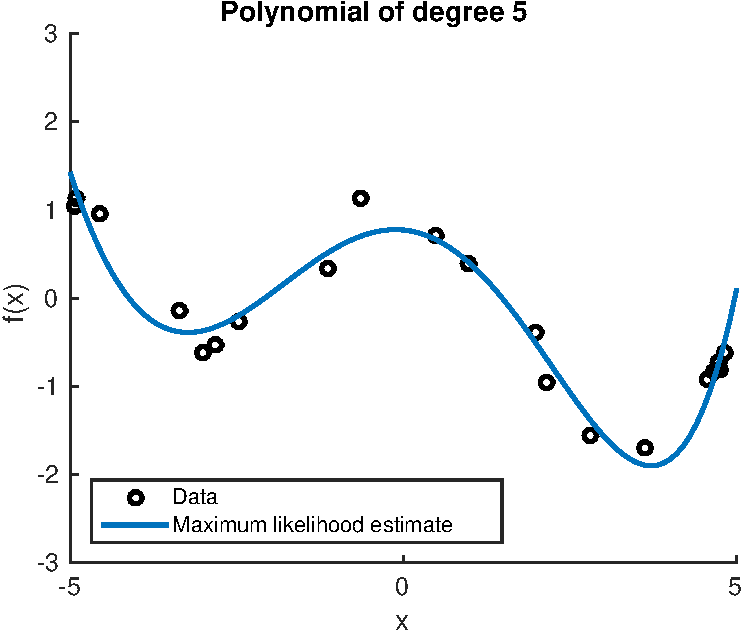
\includegraphics[width = 0.4\hsize]{./figures-intro-curvefitting/polynomial5}
 \end{figure}
 
 \vspace{-1mm}
 \begin{itemize}
 \item \cemph{Training the model} means finding parameters $\vec\theta^*$, such
   that $f(\vec x_i,\vec\theta^*)\approx y_i$
 \item Define a \cemph{loss function}, e.g., $\sum_{i=1}^N(y_i - f(\vec x_i,
   \vec\theta))^2$, which we want to optimize% \\
   % \arrow \cemph{Maximum likelihood estimation} does this implicitly
 \item Adjust $\vec\theta$ until loss is as small as we can get it: \emph{Minimisation} / \emph{optimisation}.
 \end{itemize}
\end{frame}


%%%%%%%%%%%%%%%%%%%%%%%%%%%%%%%%%%%%%%%%%
\begin{frame}{Example: Minimising the loss}
 \begin{figure}
   \centering
   \only<1>{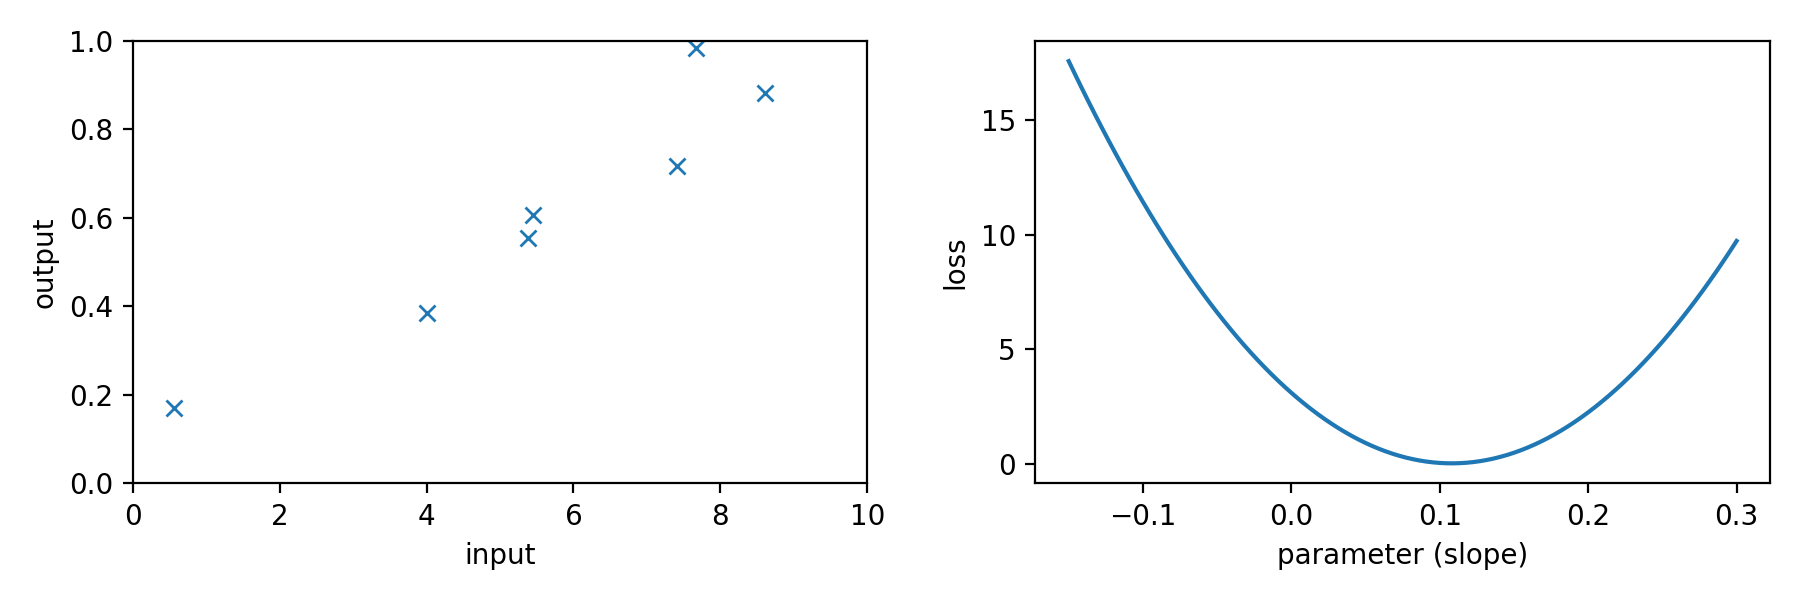
\includegraphics[width=\hsize]{./figures-vectorcalc/linreg-problem.png}}
   \only<2>{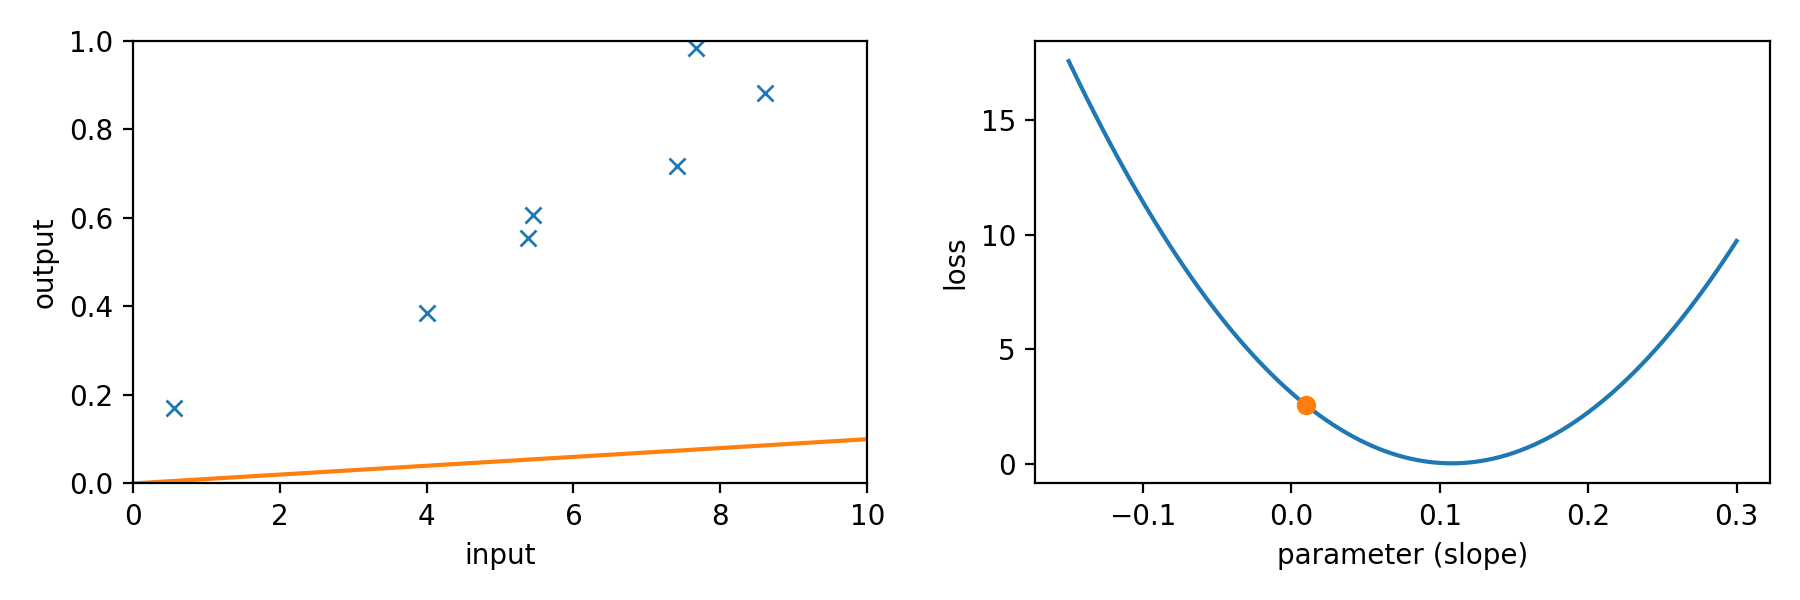
\includegraphics[width=\hsize]{./figures-vectorcalc/linreg-loss-0.png}}
   \only<3>{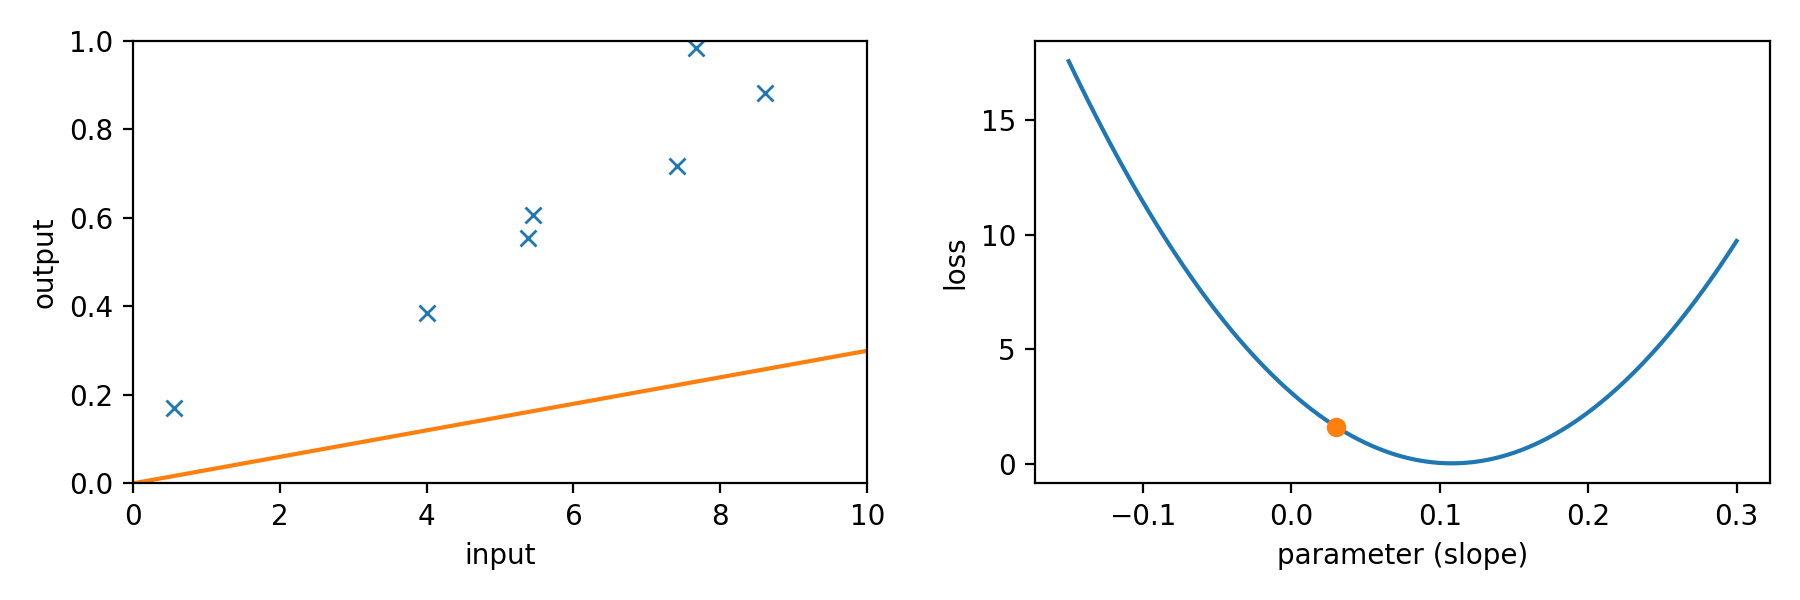
\includegraphics[width=\hsize]{./figures-vectorcalc/linreg-loss-1.png}}
   \only<4>{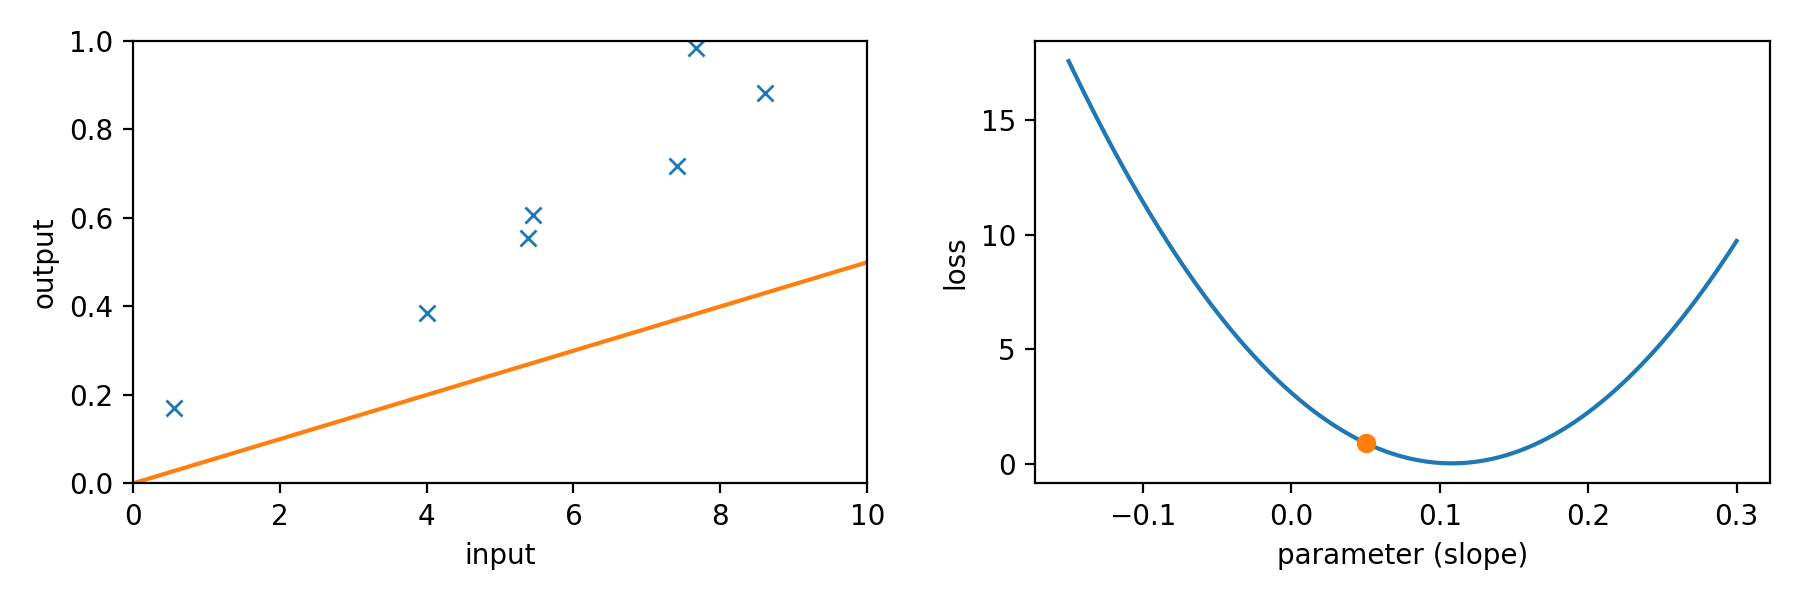
\includegraphics[width=\hsize]{./figures-vectorcalc/linreg-loss-2.png}}
   \only<5>{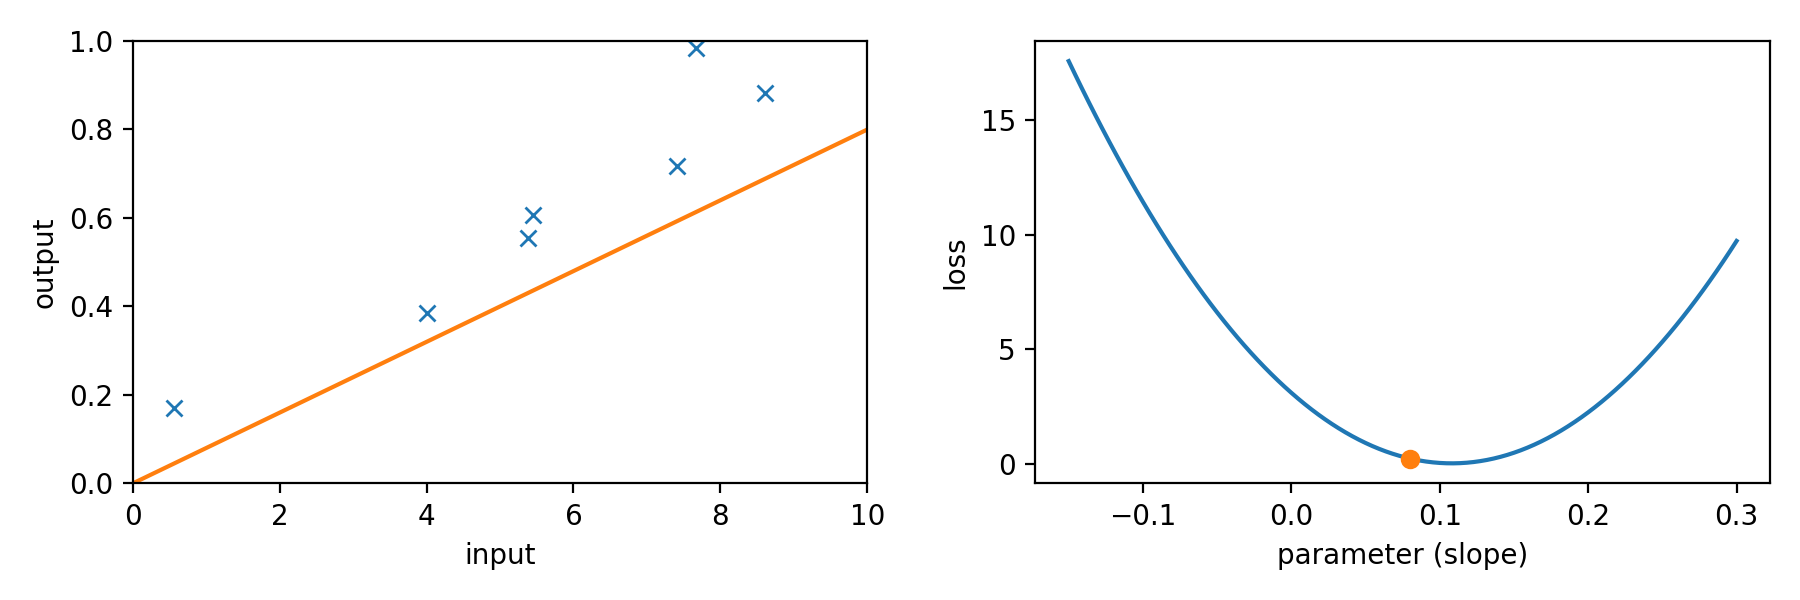
\includegraphics[width=\hsize]{./figures-vectorcalc/linreg-loss-3.png}}
   \only<6>{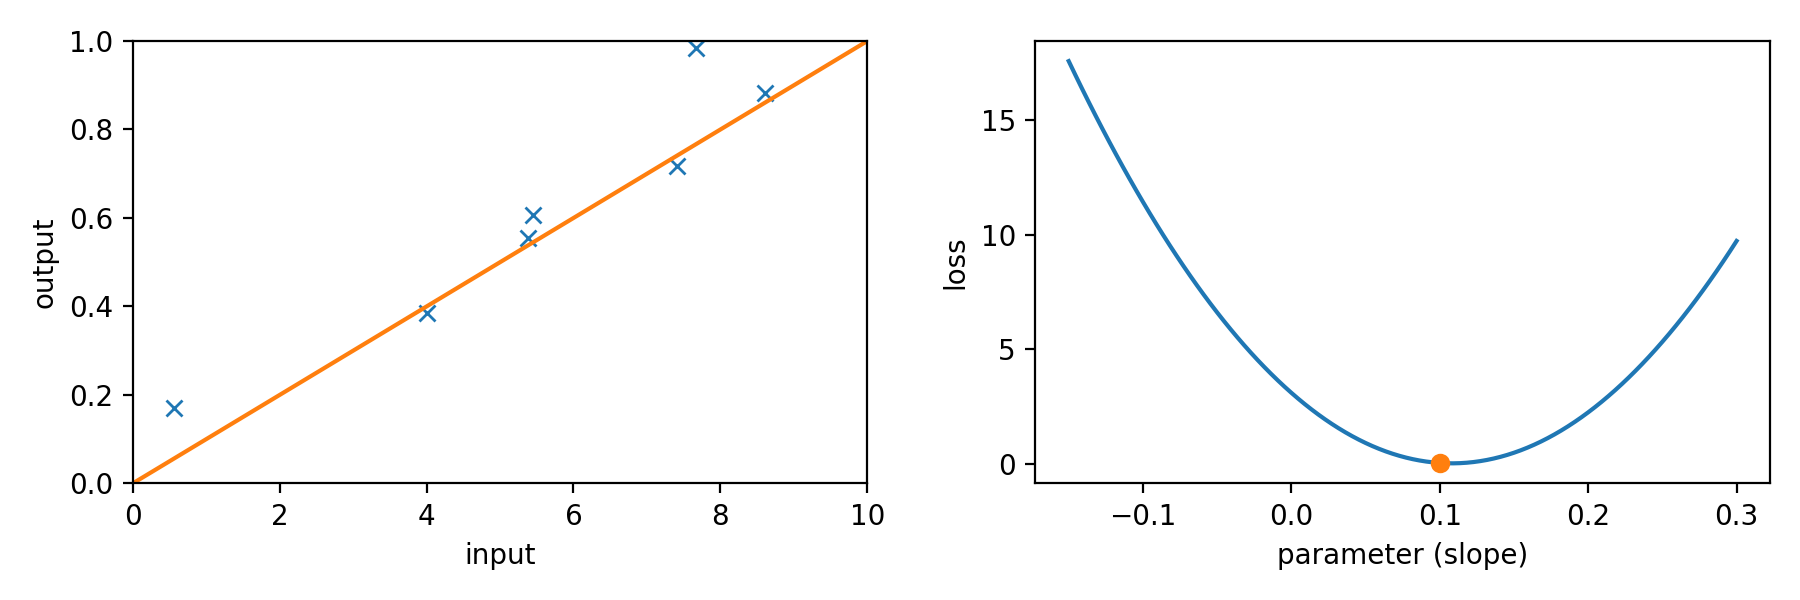
\includegraphics[width=\hsize]{./figures-vectorcalc/linreg-loss-4.png}}
   \only<7>{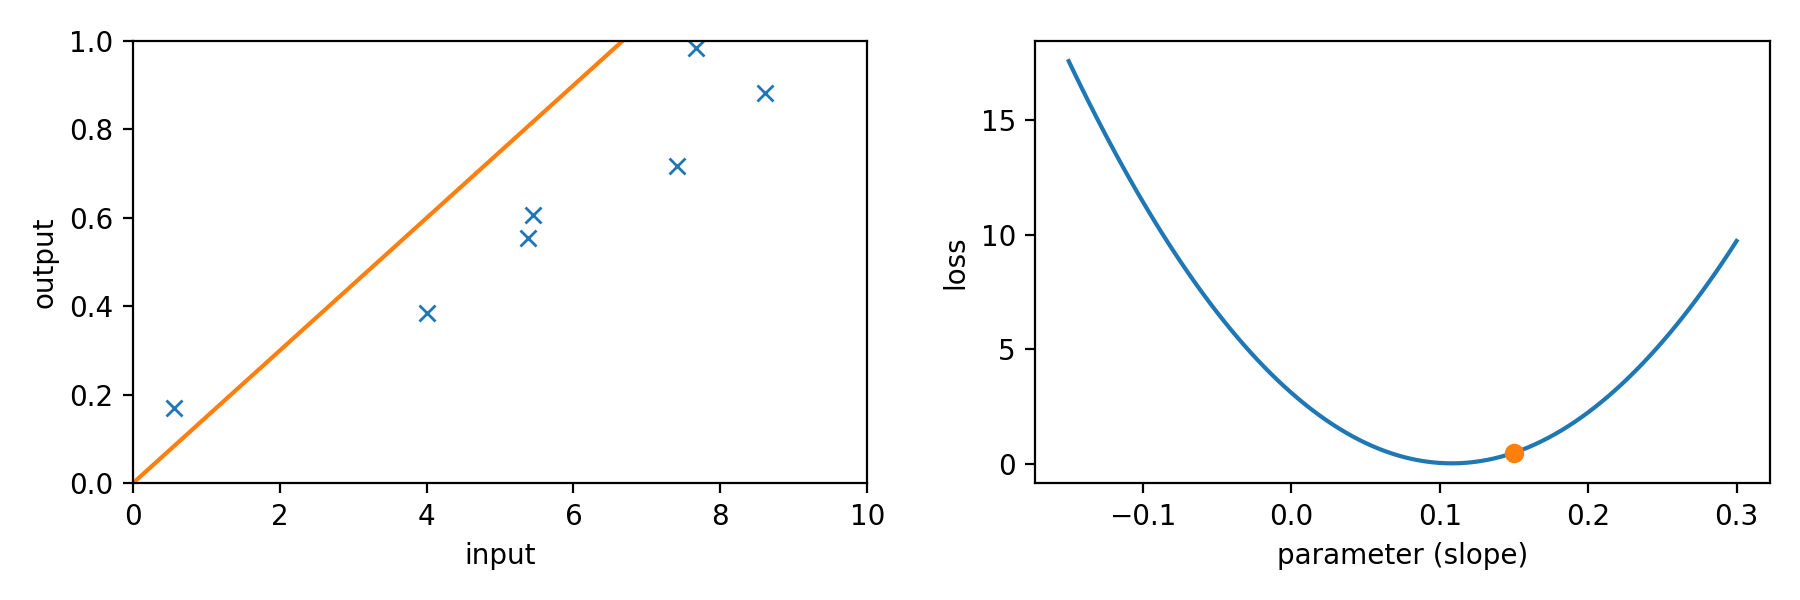
\includegraphics[width=\hsize]{./figures-vectorcalc/linreg-loss-5.png}}
   \only<8>{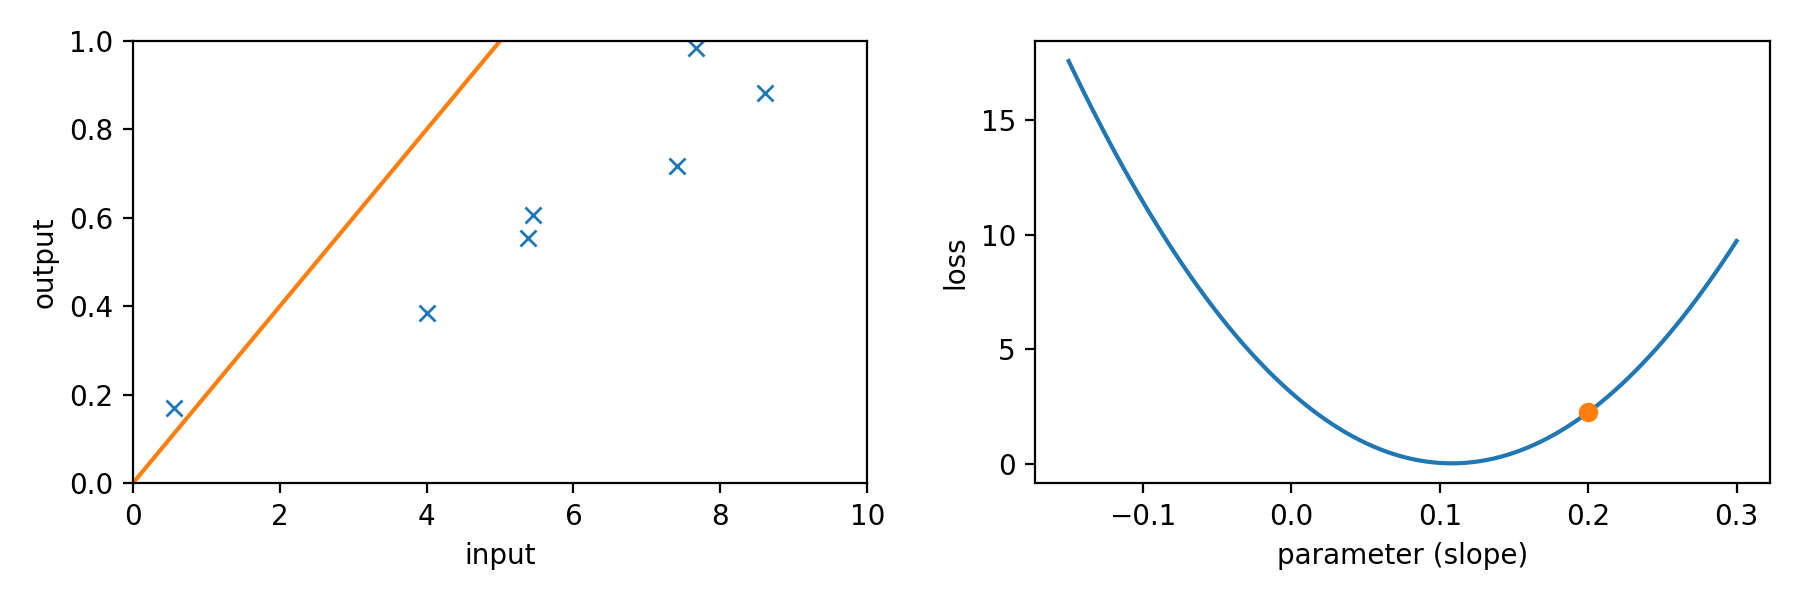
\includegraphics[width=\hsize]{./figures-vectorcalc/linreg-loss-6.png}}
   \only<9>{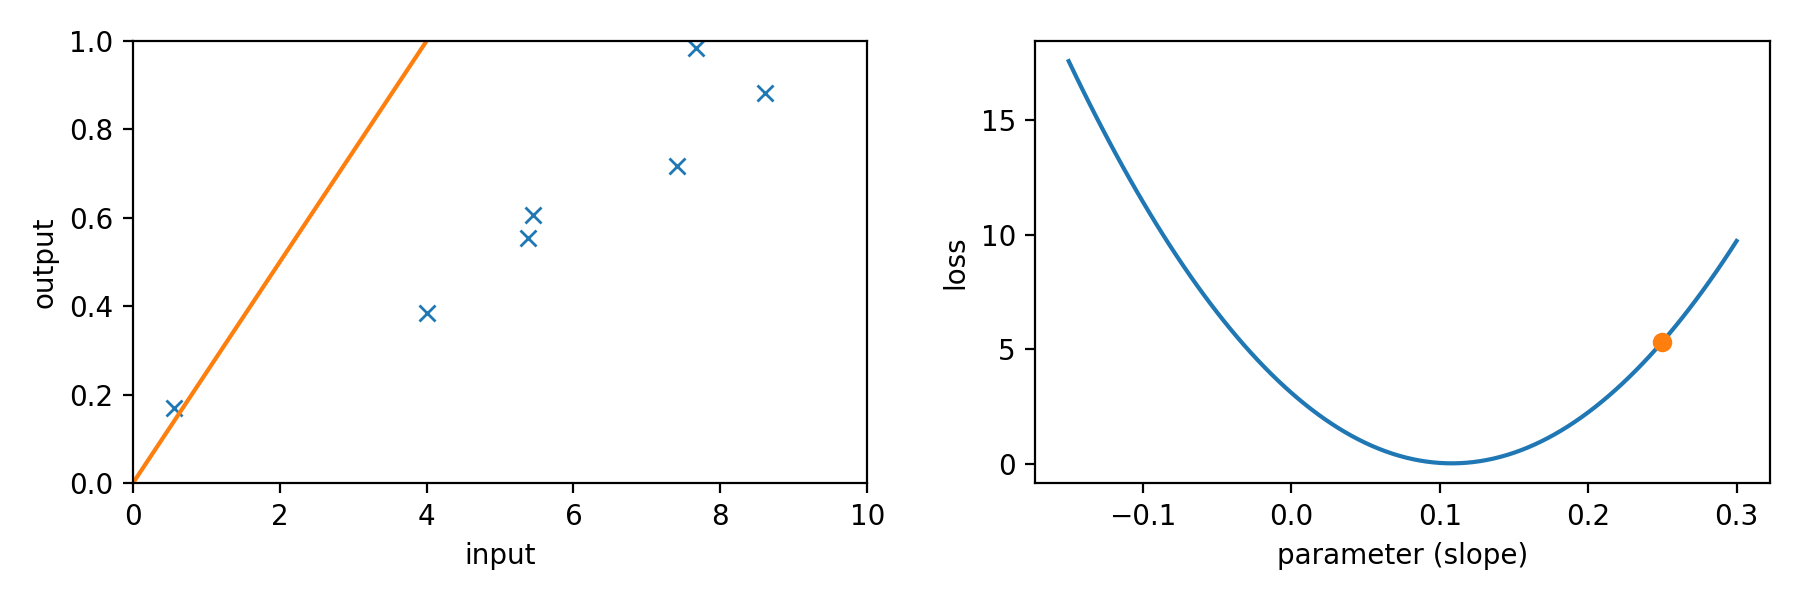
\includegraphics[width=\hsize]{./figures-vectorcalc/linreg-loss-7.png}}
   \only<10>{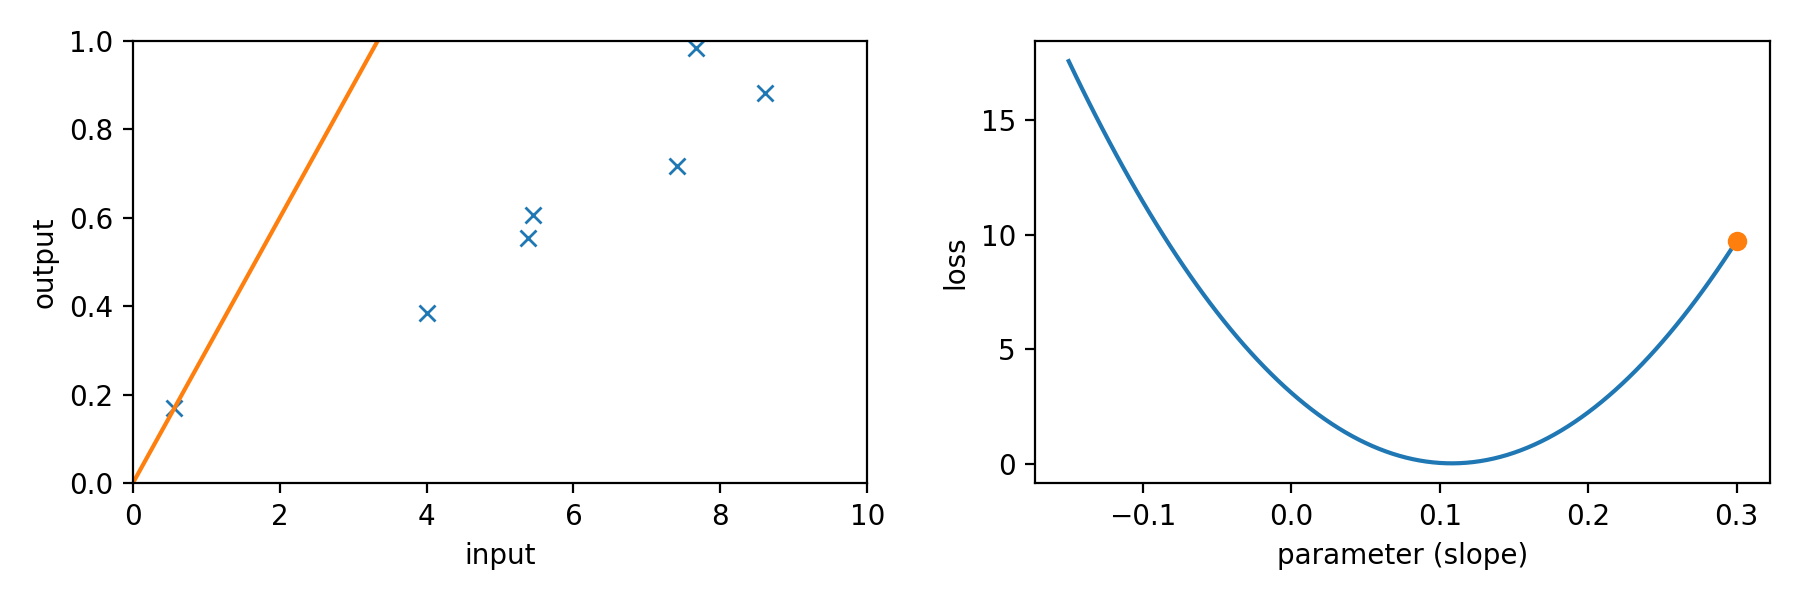
\includegraphics[width=\hsize]{./figures-vectorcalc/linreg-loss-8.png}}
 \end{figure}
\begin{align}
f(x) = a\cdot x && L(a) = \sum_{n=1}^N (f(x_n, a) - y_n)^2
\end{align}
\begin{center}
Let's adjust $a$.
\end{center}
\end{frame}



%%%%%%%%%%%%%%%%%%%%%%%%%%%%%%%%%%%%%%%%%
\begin{frame}{Example: Minimising the loss}
 \begin{figure}
   \centering
   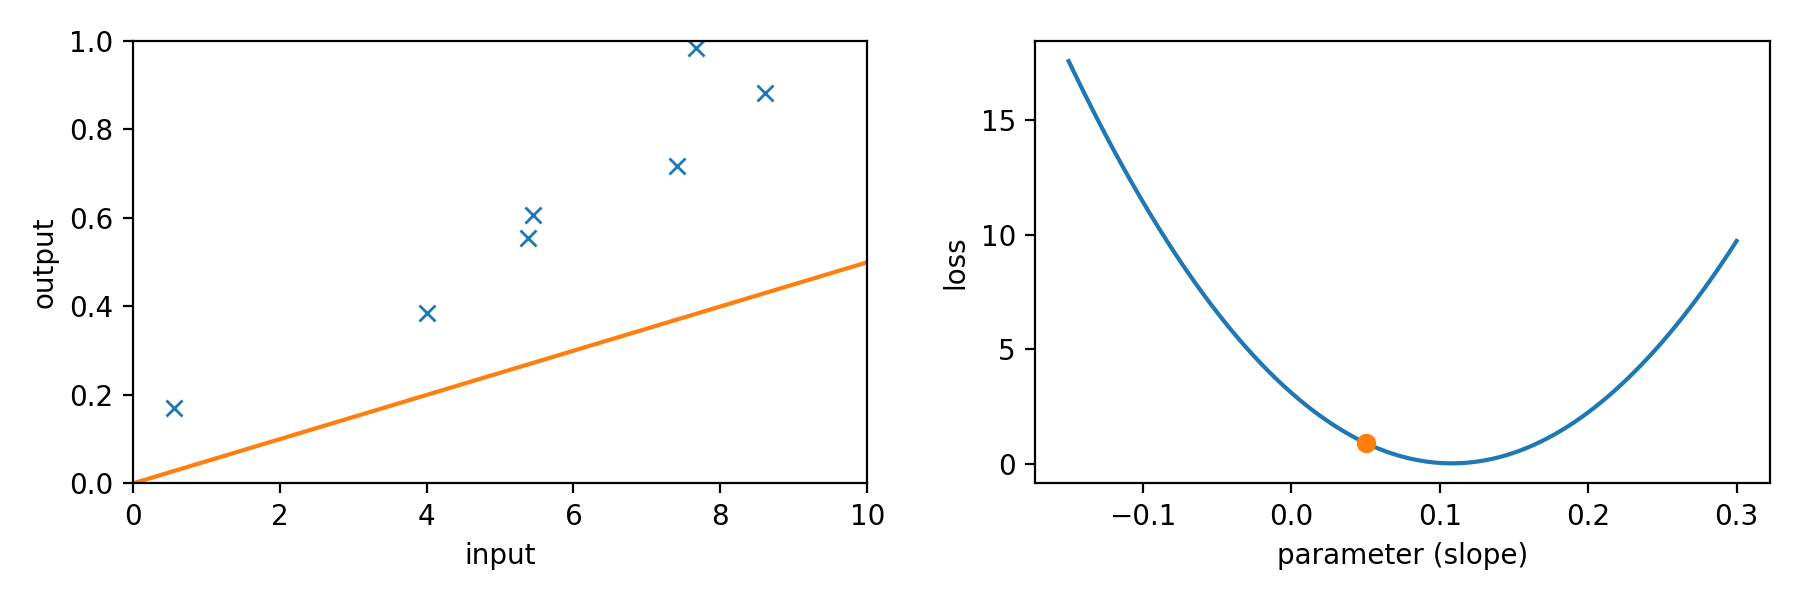
\includegraphics[width=\hsize]{./figures-vectorcalc/linreg-loss-2.png}
 \end{figure}
Two questions for now:
\begin{itemize}
\item How should we change $a$ to make the loss smaller?
\item How do we know when we can't get better?
\end{itemize}
\end{frame}





% \begin{frame}
% \frametitle{Types of Differentiation}

% \begin{enumerate}
% \item Scalar differentiation: $f:\R\to\R$ \\ \qquad \qquad \colchar{$y \in \R \text{ w.r.t. } x \in \R$}{green}
% \item Multivariate case: $f:\R^N\to\R$ \\ \qquad \qquad \colchar{$y \in \R \text{ w.r.t. vector } \vec x \in \R^N$}{green}
% \item Vector fields: $f:\R^N\to\R^M$ \\ \qquad \qquad \colchar{$\text{vector } \vec y \in \R^M \text{ w.r.t. vector } \vec x \in \R^N$}{green}
% \item General derivatives: $f:\R^{M\times N}\to \R^{P\times Q}$ \\
%   \qquad \qquad \colchar{$\text{matrix } \vec y \in \R^{P \times Q}
%     \text{ w.r.t. matrix }\mat X \in \R^{M \times N}$}{green}
% \end{enumerate}


% \end{frame}


\section{Differentiation w.r.t.~scalars}




%%%%%%%%%%%%%%%%%%%%%%%%%%%%%%%%%%%%%%%%%
\begin{frame}
  \frametitle{Scalar Differentiation $f: \R\to\R$}

% \begin{figure}
%   \centering
%   \includegraphics[width = 0.6\hsize]{./figures/finite_differences}
% \end{figure}

\begin{itemize}
\item Derivative defined as the limit of the difference quotient
%
$$
f^\prime(x) = \frac{df}{dx} = \lim_{h\to 0} \frac{f(\colchar{$x + h$}{red}) - f(x)}{h}
$$
\arrow Slope of the secant line through $f(x)$ and
$f(x+h)$
\end{itemize}
\begin{center}
  \animategraphics[loop,
  width=0.6\hsize]{10}{./figures-vectorcalc/finite-diff-animation/finite_diff_step_}{99}{0}
\end{center}

\end{frame}

%%%%%%%%%%%%%%%%%%%%%%%%%%%%%%%%%%%%%%%%%
\begin{frame}
\frametitle{Some Examples}
$$
\begin{array}{ll}
  f(x) = x^n\qquad & f^\prime(x) = nx^{n-1}\\
  f(x) = \sin(x)\qquad & f^\prime(x) = \cos(x)\\
  f(x) = \tanh(x) \qquad& f^\prime(x) = 1-\tanh^2(x)\\
  f(x) = \exp(x) \qquad &f^\prime(x) = \exp(x)\\
  f(x) = \log(x) \qquad &f^\prime(x) = \frac{1}{x}
\end{array}
$$
\end{frame}


%%%%%%%%%%%%%%%%%%%%%%%%%%%%%%%%%%%%%%%%%
\begin{frame}
  \frametitle{Differentiation Rules}

  \begin{itemize}[<+->]
  \item Sum Rule
    $$\big(f(x)+g(x)\big)^\prime = \green{f^\prime(x)} + \blue{g^\prime(x)} =
    \green{\frac{df(x)}{dx}} + \blue{\frac{dg(x)}{dx}}$$
  \item Product Rule
    $$
    \big(f(x) g(x)\big)^\prime = \green{f^\prime(x)g(x)} + \blue{f(x)g^\prime(x)} =
    \green{\frac{df(x)}{dx}g(x)} + \blue{f(x) \frac{d g(x)}{dx}}
    $$
  \item Chain Rule
    $$
     (g\circ f)^\prime(x) =  \big(g(f(x))\big)^\prime
     =\green{g^\prime(f(x))}\blue{f^\prime(x)} = \green{\frac{dg(f(x))}{df}}\blue{\frac{df(x)}{dx}}
    $$
   \item Quotient Rule
   	$$
   	\Big(\frac{f(x)}{g(x)}\Big)^\prime = \frac{\green{f(x)^\prime g(x)} - \blue{f(x)g(x)^\prime}}{\green{(g(x))^2}} = \frac{\blue{\frac{df}{dx}g(x)} - \green{f(x)\frac{dg}{dx}}}{\green{(g(x))^2}}
   	$$
  \end{itemize}
\end{frame}


%%%%%%%%%%%%%%%%%%%%%%%%%%%%%%%%%%%%%%%%%
\begin{frame}
\frametitle{Example: Scalar Chain Rule}
$$
     (g\circ f)^\prime(x) =  \big(g(f(x))\big)^\prime
     =\green{g^\prime(f(x))}\blue{f^\prime(x)} = \green{\frac{dg}{df}}\blue{\frac{df}{dx}}
    $$
    
\begin{columns}[t]

\column{0.50\hsize}
\begin{center}
\textbf{Beginner}
\end{center}
\vspace{-6mm}

\begin{align*}
  g(z) &= 6z + 3\\
  z &= f(x) = -2x + 5 \\
  (g\circ f)^\prime(x) &= \onslide+<2->{\green{\underbrace{(6)}_{dg/df}}\blue{\underbrace{(-2)}_{df/dx}} \\ &= -12}
\end{align*}


\column{0.60\hsize}
\begin{center}
\textbf{Advanced}
\end{center}
\vspace{-6mm}

\begin{align*}
%  f(x) = \frac{\exp(x) + \exp(-x)}{\exp(x)}\\
  g(z) &= \tanh(z)\\
  z &= f(x) = x^n \\
  (g\circ f)^\prime(x) &= \onslide+<2->{\green{\underbrace{\big(1-\tanh^2(x^{n}))}_{dg/df}}\blue{\underbrace{nx^{n-1}}_{df/dx}}}
\end{align*}

\end{columns}
\onslide+<1>{
\vspace{-4mm}
\begin{center}
\textbf{Work it out with your neighbors}
\end{center}}
\end{frame}



\begin{frame}{Finding minima}
\vspace{-0.4cm}
 \begin{figure}
   \centering
   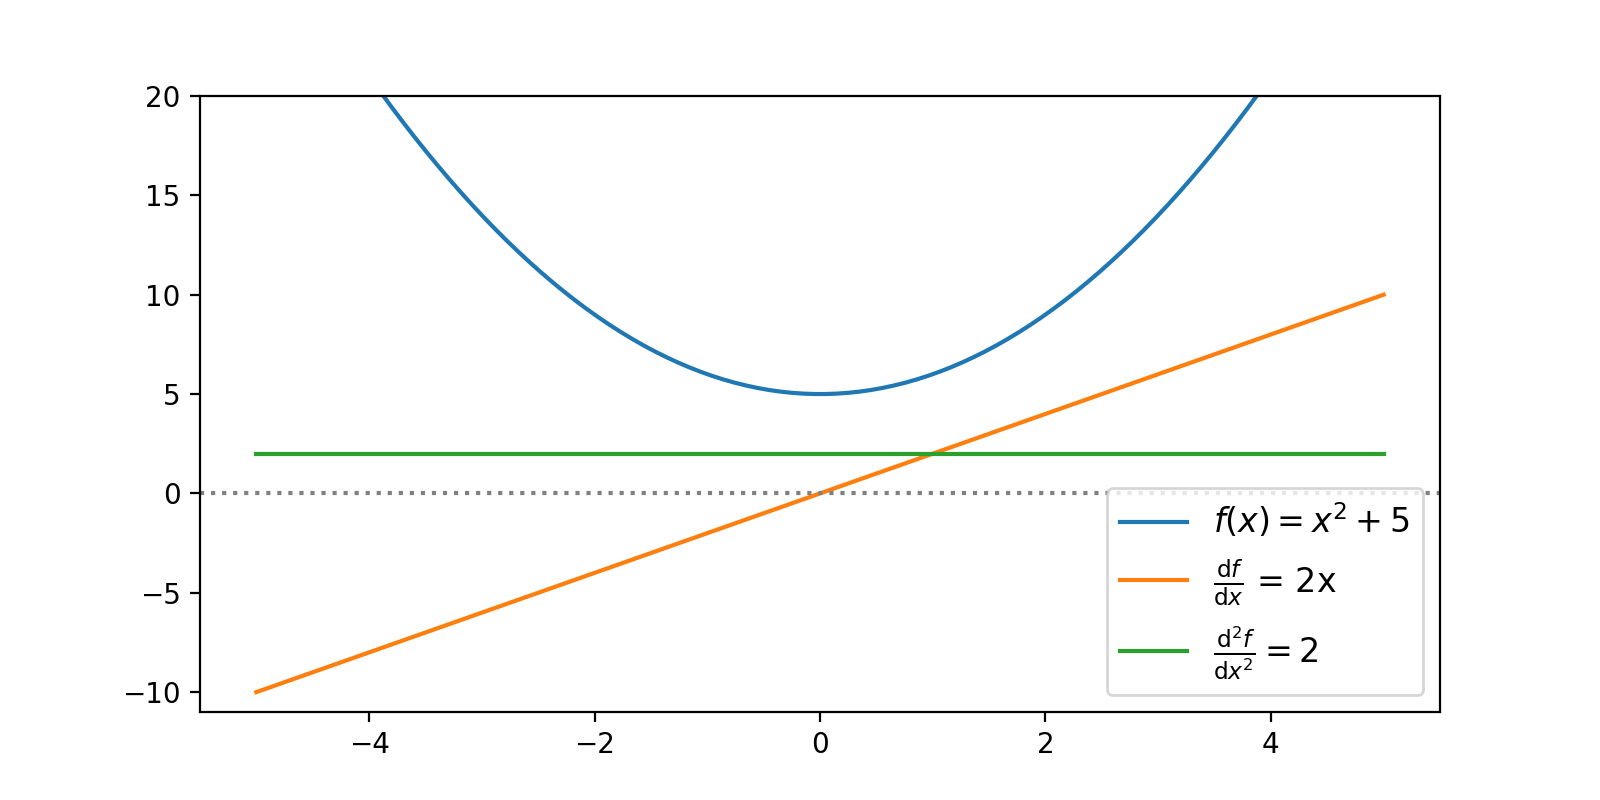
\includegraphics[width=0.85\hsize]{./figures-vectorcalc/gradient-example.png}
 \end{figure}
\vspace{-0.4cm}
Q1: How should we change the input to reduce the output? \pause \\
% The derivative tells us how the function changes if we increase the input. So: \pause
\begin{itemize}
\item Find the derivative function and compute it at a point to find the point's gradient. \pause
\item Increase for negative gradients. Decrease for positive gradients. \pause
\end{itemize}
This is the idea behind \emph{gradient descent}.
\end{frame}



\begin{frame}[allowframebreaks]{Finding minima}
\vspace{-0.4cm}
 \begin{figure}
   \centering
   \only<1,3>{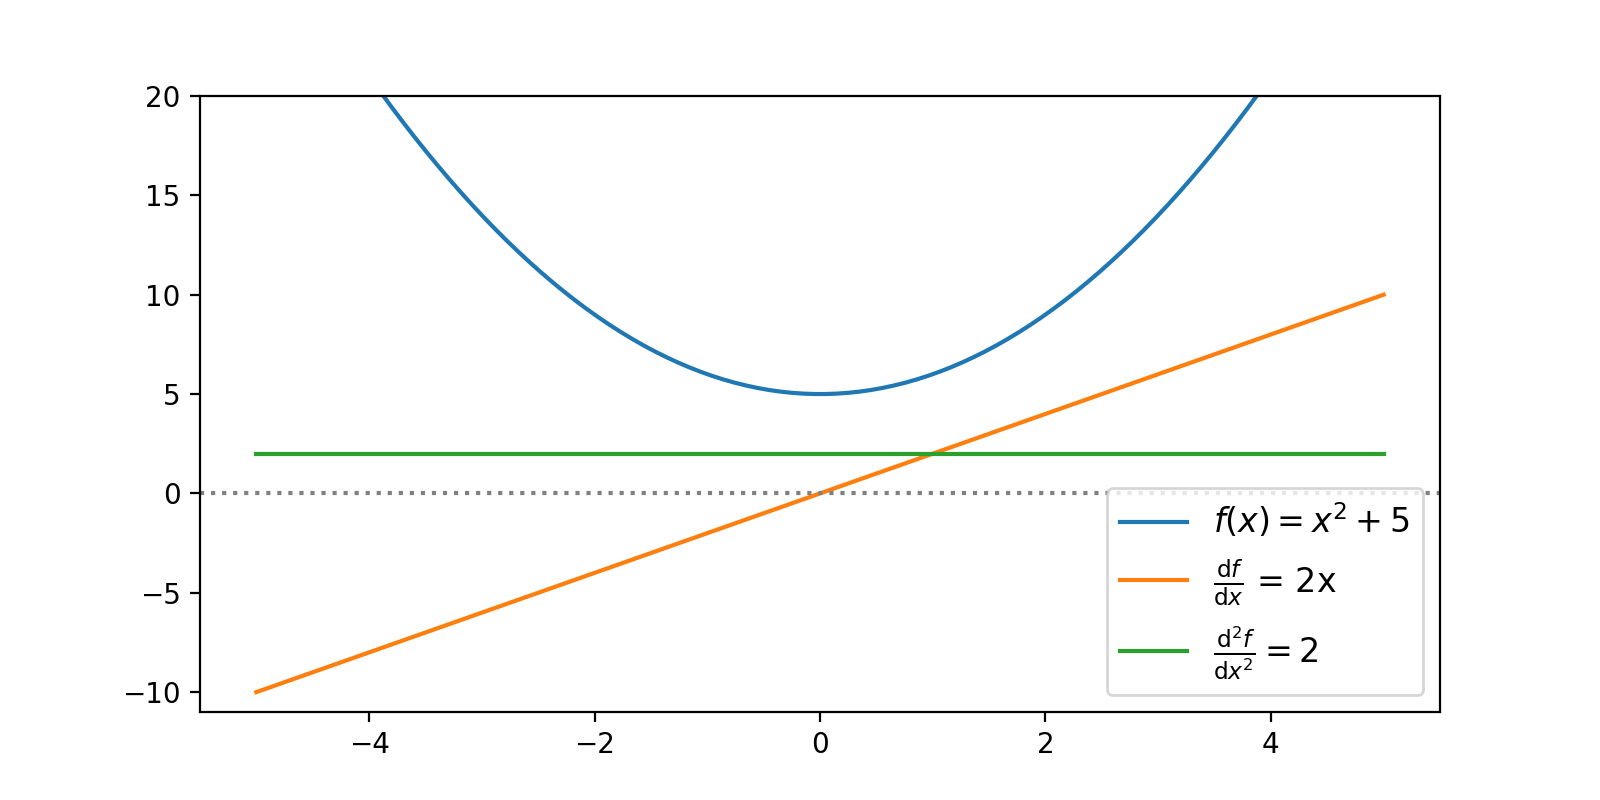
\includegraphics[width=0.85\hsize]{./figures-vectorcalc/gradient-example.png}}
   \only<2>{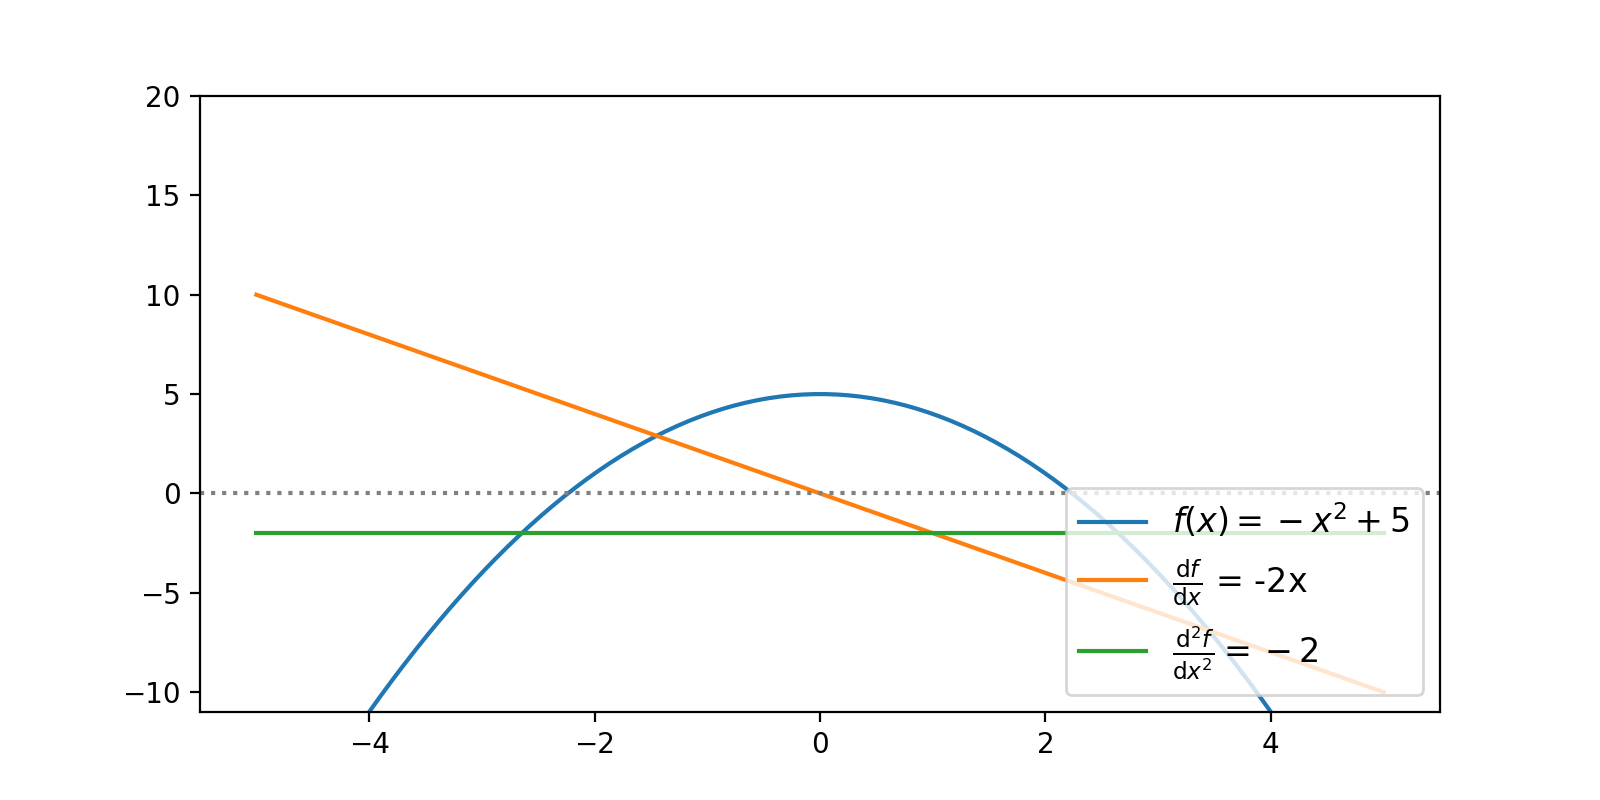
\includegraphics[width=0.85\hsize]{./figures-vectorcalc/gradient-example-max.png}}
 \end{figure}
\vspace{-0.4cm}
\begin{itemize}
\item At a minimum, there is no change we can make that lowers our function value $\implies$ gradient must be zero. \pause
\item Zero gradient is not enough! \pause
\item For minimum, $f(x)$ must go from decreasing to increasing \\
$\implies$ gradient of gradient positive
\end{itemize}
\end{frame}


\begin{frame}{Local and global minima}
Board.
\end{frame}



\begin{frame}{Example: Linear regression}
For the example from earlier, find optimal $a$:
\begin{align}
f(x) = a\cdot x && L(a) = \sum_{n=1}^N (f(x_n) - y_n)^2
\end{align} \pause
\begin{align}
\deriv[L]{a} = \sum_{n=1}^N 2 (a x_n - y_n) x_n = \sum_{n=1}^N 2ax_n^2 - 2x_ny_n = 0
\end{align} \pause
\begin{align}
2a \sum_n x_n^2 = \sum_n2x_ny_n
\end{align} \pause
\begin{align}
a = \frac{\sum_nx_ny_n}{\sum_n x_n^2}
\end{align} \pause
\begin{align}
\frac{\mathrm{d}^2L}{\mathrm{d}a^2} = \sum_{n=1}^N 2x_n^2 \geq 0
\end{align}
\end{frame}


\begin{frame}{Summary}
You have seen:
\begin{itemize}
\item That derivatives are useful for finding minima of functions \pause
\item How to differentiate simple functions \pause
\item An example of solving for the minimum point \pause
\item How to identify minima
\end{itemize}

% Consider exercises 5.1-5.3 in the MML book. EXERCISES
\end{frame}

\section{Differentiation w.r.t.~vectors}

\begin{frame}{Linear regression: multiple parameters}
What happens when our function has multiple parameters?
\begin{equation}
f(x) = \theta_3 x^3 + \theta_2 x^2 + \theta_1 x + \theta_0
\end{equation} \pause

Think of a \emph{vector} as parameterising our function:
\begin{align}
f(x) = \vec\theta\transpose \vphi(x) && \vphi(x) = \begin{bmatrix}x^3 && x^2 && x && 1\end{bmatrix}\transpose
\end{align} \pause

We want to:
\begin{itemize}
\item Understand how a function (e.g.~loss) changes when we change $\vec\theta$. \pause
\item Characterise what an optimum is for a function of a vector.
\end{itemize} \pause

\begin{center}
Both can be analysed by \\ turning the multi-D problem into many 1D problems.
\end{center}
\end{frame}

\begin{frame}{Directional derivative}

 \begin{figure}
   \centering
   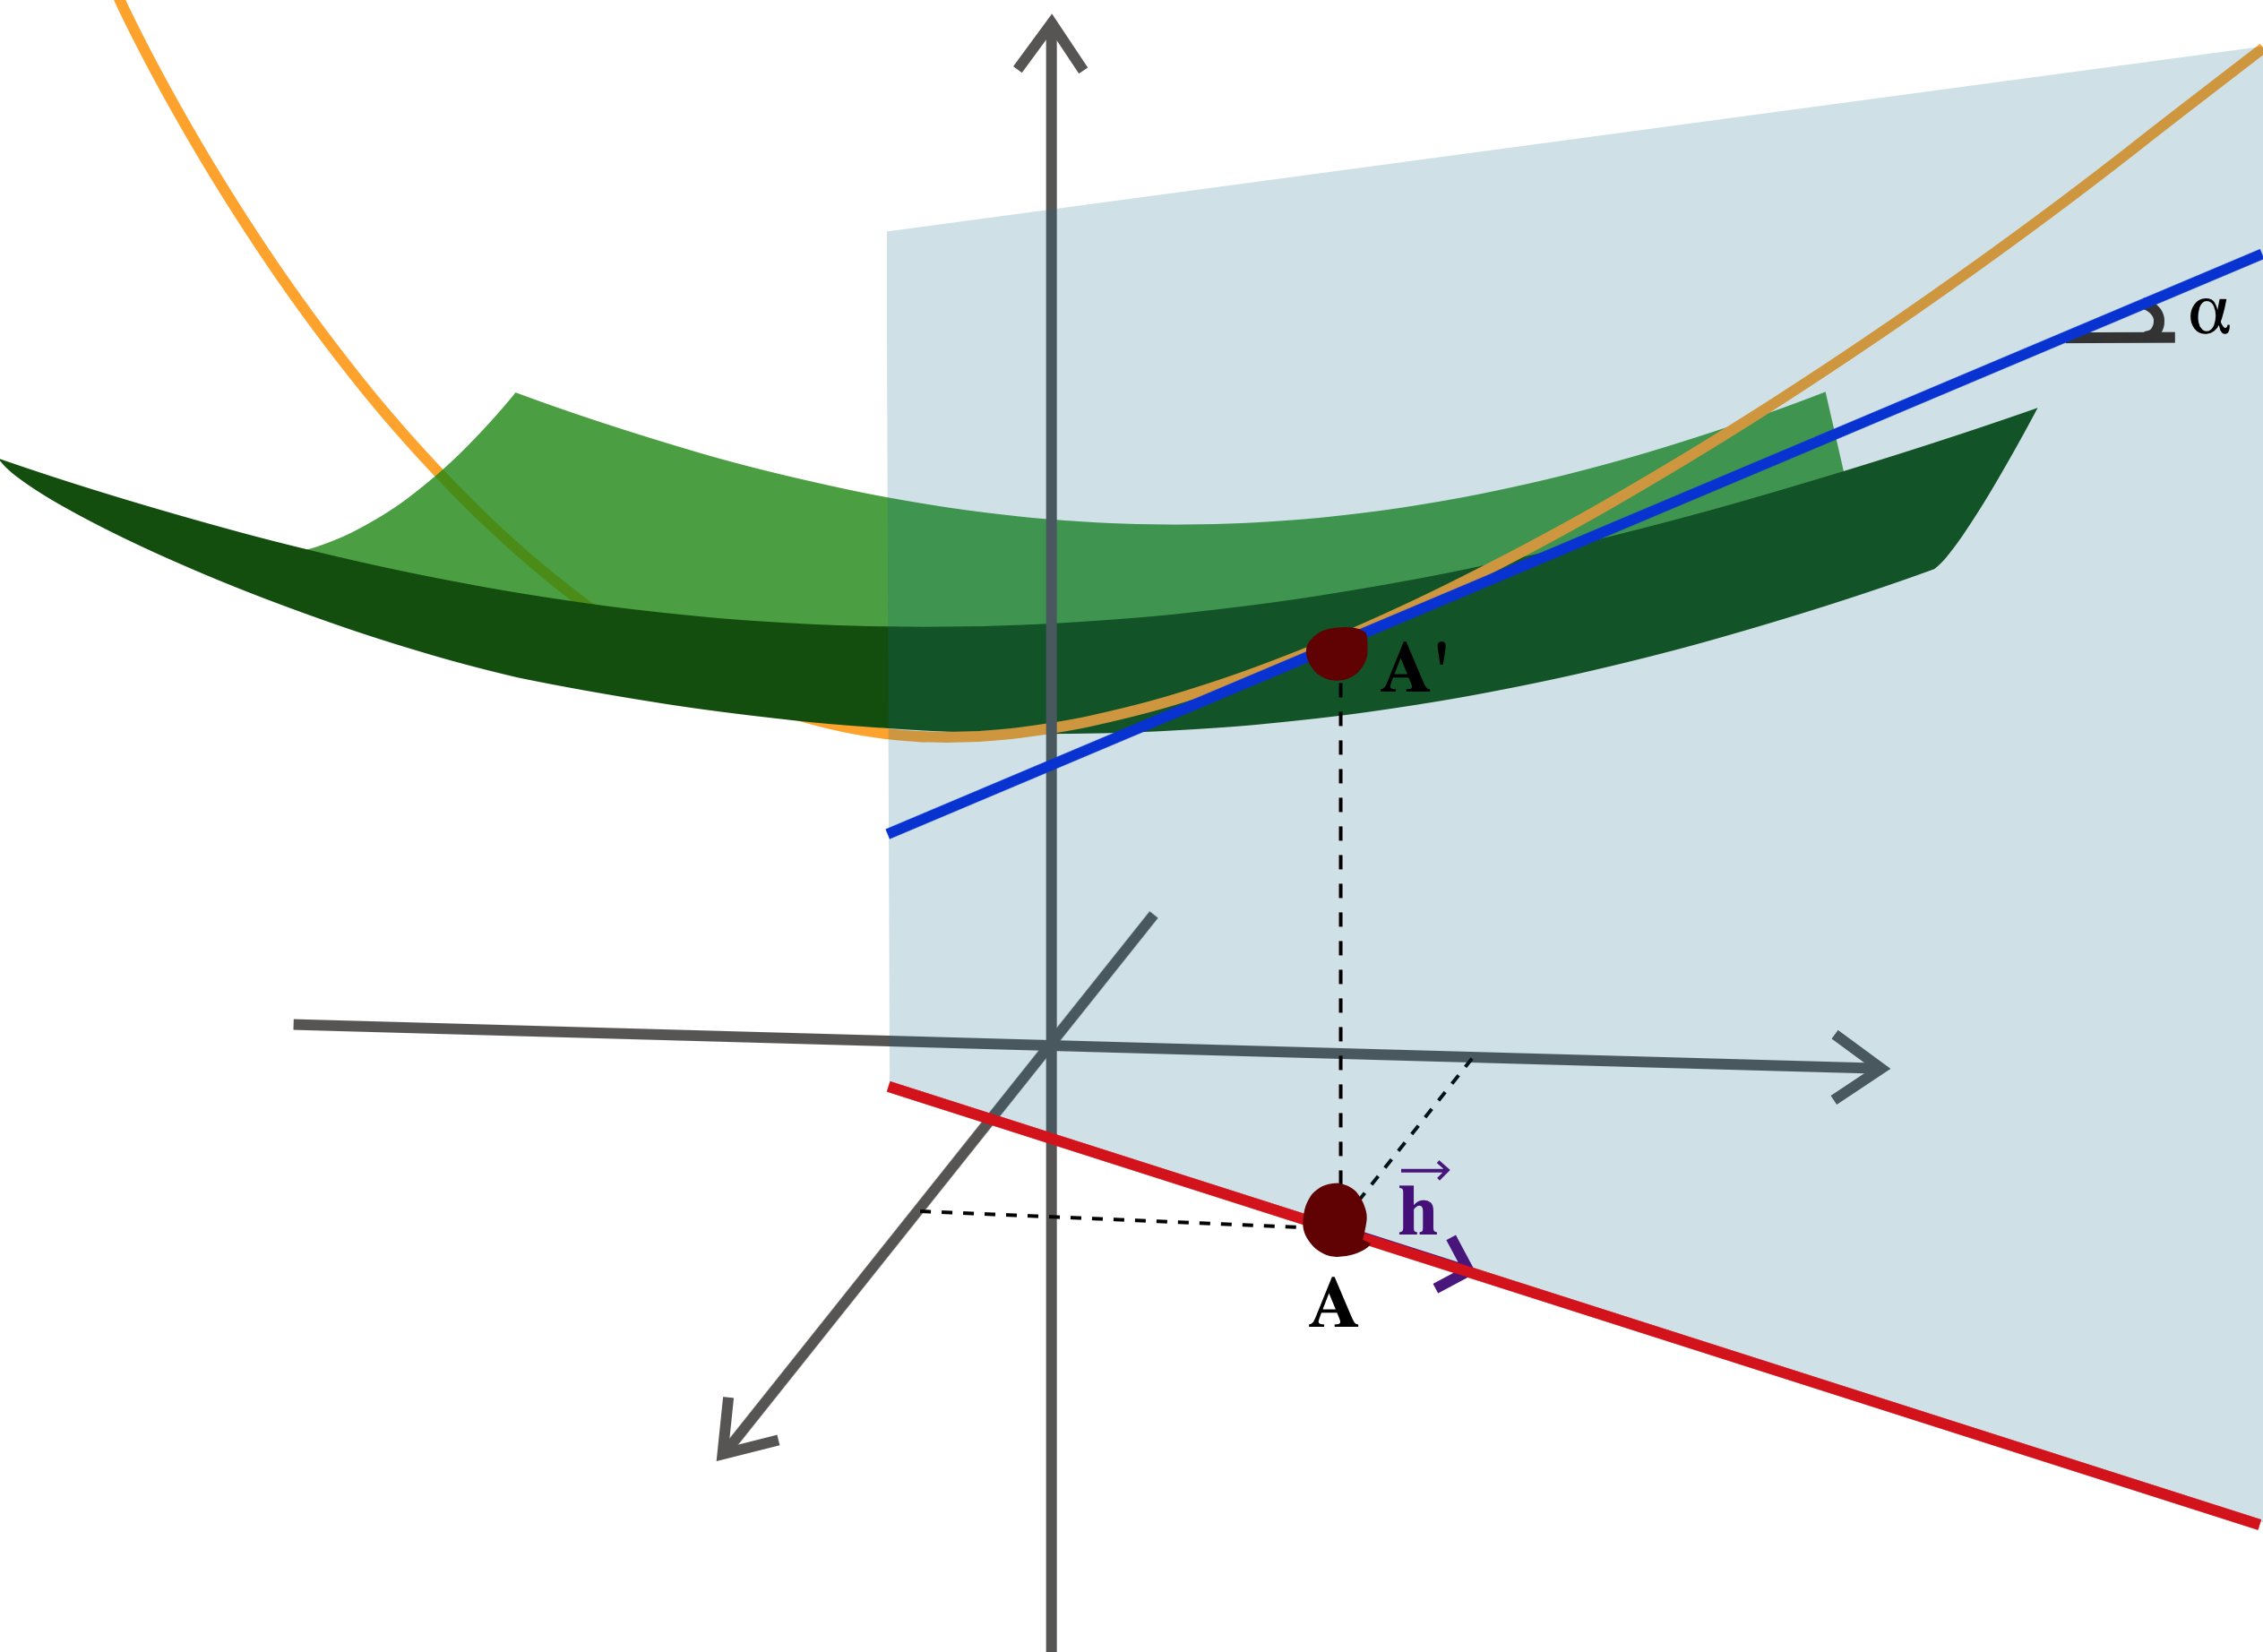
\includegraphics[width=0.7\hsize]{./figures-vectorcalc/directional-deriv.png}
 \end{figure}

 How does the function change if we move in a particular \textit{direction}?
\end{frame}

\begin{frame}{Directional derivative}
Define \emph{directional derivative} $\nabla_\vv L(\vtheta)$ as how much the function changes if we move in direction $\vv$:
\only<1>{
\begin{align*}
\nabla_\vv L(\vtheta) = \lim_{h\to 0} \frac{L(\vtheta + h\vv) - L(\vtheta)}{h}
\end{align*}}
\only<2->{\begin{equation*}
\nabla_\vv L(\vtheta) = \lim_{h\to 0} \frac{L(\theta_1 + hv_1, \theta_2 + hv_2) - L(\theta_1, \theta_2)}{h}
\end{equation*}} \pause\pause
\begin{equation*}
= \lim_{h\to 0} \frac{L(\theta_1 + hv_1, \theta_2 + hv_2) - {\color{blue}L(\theta_1, \theta_2  + hv_2)}}{h} + \frac{{\color{blue}L(\theta_1, \theta_2 + hv_2)} - L(\theta_1, \theta_2)}{h}
\end{equation*}\pause
\begin{equation*}
= \lim_{h\to 0} \frac{L(\theta_1 + h', \theta_2 + h'\frac{v_2}{v_1})\!-\!{\color{blue}L(\theta_1, \theta_2  + h'\frac{v_2}{v_1})}}{h'/v_1}\!+\! \frac{{\color{blue}L(\theta_1, \theta_2 + h'')}\!-\!L(\theta_1, \theta_2)}{h''/v_2}
\end{equation*}\pause
\begin{equation*}
= \pderiv[L]{\theta_1} v_1 + \pderiv[L]{\theta_2} v_2% && \qquad \text{to prove, substitute e.g.~}h' = hv_1
\end{equation*} \pause
\begin{itemize}
\item Can find gradient in \emph{any} direction with the \emph{partial derivatives}
% \item An optimum is where the gradient is zero in \emph{all directions}!
\end{itemize}
\end{frame}


%%%%%%%%%%%%%%%%%%%%%%%%%%%%%%%%%%%%%%%%%
\begin{frame}
  \frametitle{Multivariate Differentiation $f: \R^N\to\R$}

  \begin{align*}
    y = f(\vec x)\,,\quad \vec x =\begin{bmatrix}
                                    x_1\\
                                    \vdots\\
                                    x_N
                                  \end{bmatrix}\in\R^N
  \end{align*}

  \begin{itemize}[<+->]
  \item \cemph{Partial derivative} (change one coordinate at a time):
    \begin{align*}
      \frac{\partial f}{\partial x_i} = \lim_{h\to 0}
      \frac{f(x_1,\dotsc, x_{i-1}, \colchar{$x_i + h$}{red}, x_{i+1},
      \dotsc, x_N) - f(\vec x)}{h}
    \end{align*}
  \item \cemph{Jacobian} vector (\cemph{gradient}) collects all partial derivatives:
    \begin{align*}
      \diffF{f}{\vec x} =
      \begin{bmatrix}
         \frac{\partial f}{\partial x_1} & \cdots & \pdiffF{f}{x_N}
      \end{bmatrix}\in\R^{1\times N}
    \end{align*}
    Note: By convention, we define this to be a \emph{row vector}.
  \end{itemize}
  
\end{frame}


\begin{frame}{Multivariate Differentiation $f: \R^N\to\R$}
\begin{myblock}{Derivative w.r.t.~vector}
Since we can find the directional derivative \textit{in any direction} with the Jacobian, we \emph{define} this vector to be the derivative of a function w.r.t.~a vector.
\end{myblock}
\end{frame}



\begin{frame}{Steepest descent direction}
Directional derivative:
\begin{equation}
\nabla_{\vec v} f(\vtheta) = \diffF{f}{\vtheta}\vec v
\end{equation}
\vspace{-0.5cm}
\begin{center}\small(inner product, row vector times column vector)\end{center} \pause

\vspace{0.2cm}

\begin{center}
\large What is the direction where the function changes the most?
\end{center} \pause
\begin{equation}
\diffF{f}{\vtheta}\vec v = \norm{\diffF{f}{\vtheta}}\norm{\vec v} \cos \beta 
\end{equation}\pause
\begin{itemize}
\item Choose unit vector $\vec v$ \pause
\item Angle between vectors $\beta$ should be zero $\implies \cos \beta = 1$. \pause
\end{itemize}
\begin{center}
\Large Steepest descent points in direction of Jacobian/gradient vector.
\end{center}
\end{frame}


%%%%%%%%%%%%%%%%%%%%%%%%%%%%%%%%%%%%%%%%%
\begin{frame}[t]
\frametitle{Example: Multivariate Differentiation}

\vspace{-1cm}
\begin{columns}[t]

\column{0.50\hsize}
\begin{center}
\textbf{Beginner}
\end{center}
\vspace{-6mm}

\begin{align*}
  &f: \R^2 \to \R\\
  &f(x_1,x_2) = x_1^2x_2+x_1x_2^3\in\R
\end{align*}

\column{0.50\hsize}
\begin{center}
\textbf{Advanced}
\end{center}
\vspace{-6mm}

\begin{align*}
 &f: \R^2 \to \R\\
  &f(x_1,x_2) = (x_1 + 2x_2^3)^2\in\R
\end{align*}

\end{columns}

\begin{center}
Partial derivatives\visible<1>{? Gradient?}  \\
\visible<1>{\textbf{Work it out with your neighbors}}
\end{center}
\vspace{-1.35cm}

\pause
\begin{columns}[t]

\column{0.5\hsize}
\begin{align*}
\frac{\partial f(x_1,x_2)}{\partial x_1} &= 2x_1x_2 + x_2^3\\
\frac{\partial f(x_1,x_2)}{\partial x_2} &= x_1^2+3x_1x_2^2
\end{align*}

\column{0.5\hsize}
\vspace{-4mm}
\begin{align*}
\frac{\partial f(x_1,x_2)}{\partial x_1} &= 2(x_1 + 2x_2^3)\green{\overbrace{(1)}^{\pdiffF{}{x_1}(x_1 + 2x_2^3)}}\\
\frac{\partial f(x_1,x_2)}{\partial x_2} &= 2(x_1 + 2x_2^3)\blue{\underbrace{(6x_2^2)}_{\pdiffF{}{x_2}(x_1 + 2x_2^3)}}\\
\end{align*}

\end{columns}

\pause
\vspace{-1cm}
\begin{align*}
\text{Gradient}\qquad
\diffF{f}{\vec x} =
  \begin{bmatrix}
\frac{\partial f(x_1,x_2)}{\partial x_1} & \frac{\partial
  f(x_1,x_2)}{\partial x_2}
\end{bmatrix} \in\R^{1\times 2}\,
\end{align*}
\vspace{-1.35cm}

\begin{columns}[t]

\column{0.5\hsize}
\begin{align*}
  \diffF{f}{\vec x} =
\begin{bmatrix}
 2x_1x_2 + x_2^3 & x_1^2+3x_1x_2^2
\end{bmatrix}
\end{align*}

\column{0.5\hsize}
\begin{align*}
  \diffF{f}{\vec x} =
\begin{bmatrix}
 2(x_1 + 2x_2^3) & 12(x_1 + 2x_2^3)x_2^2
\end{bmatrix}
\end{align*}

\end{columns}

\end{frame}


\begin{frame}{Optima, minima, maxima}
What is an optimum for a function of a vector?
 \begin{figure}
   \centering
   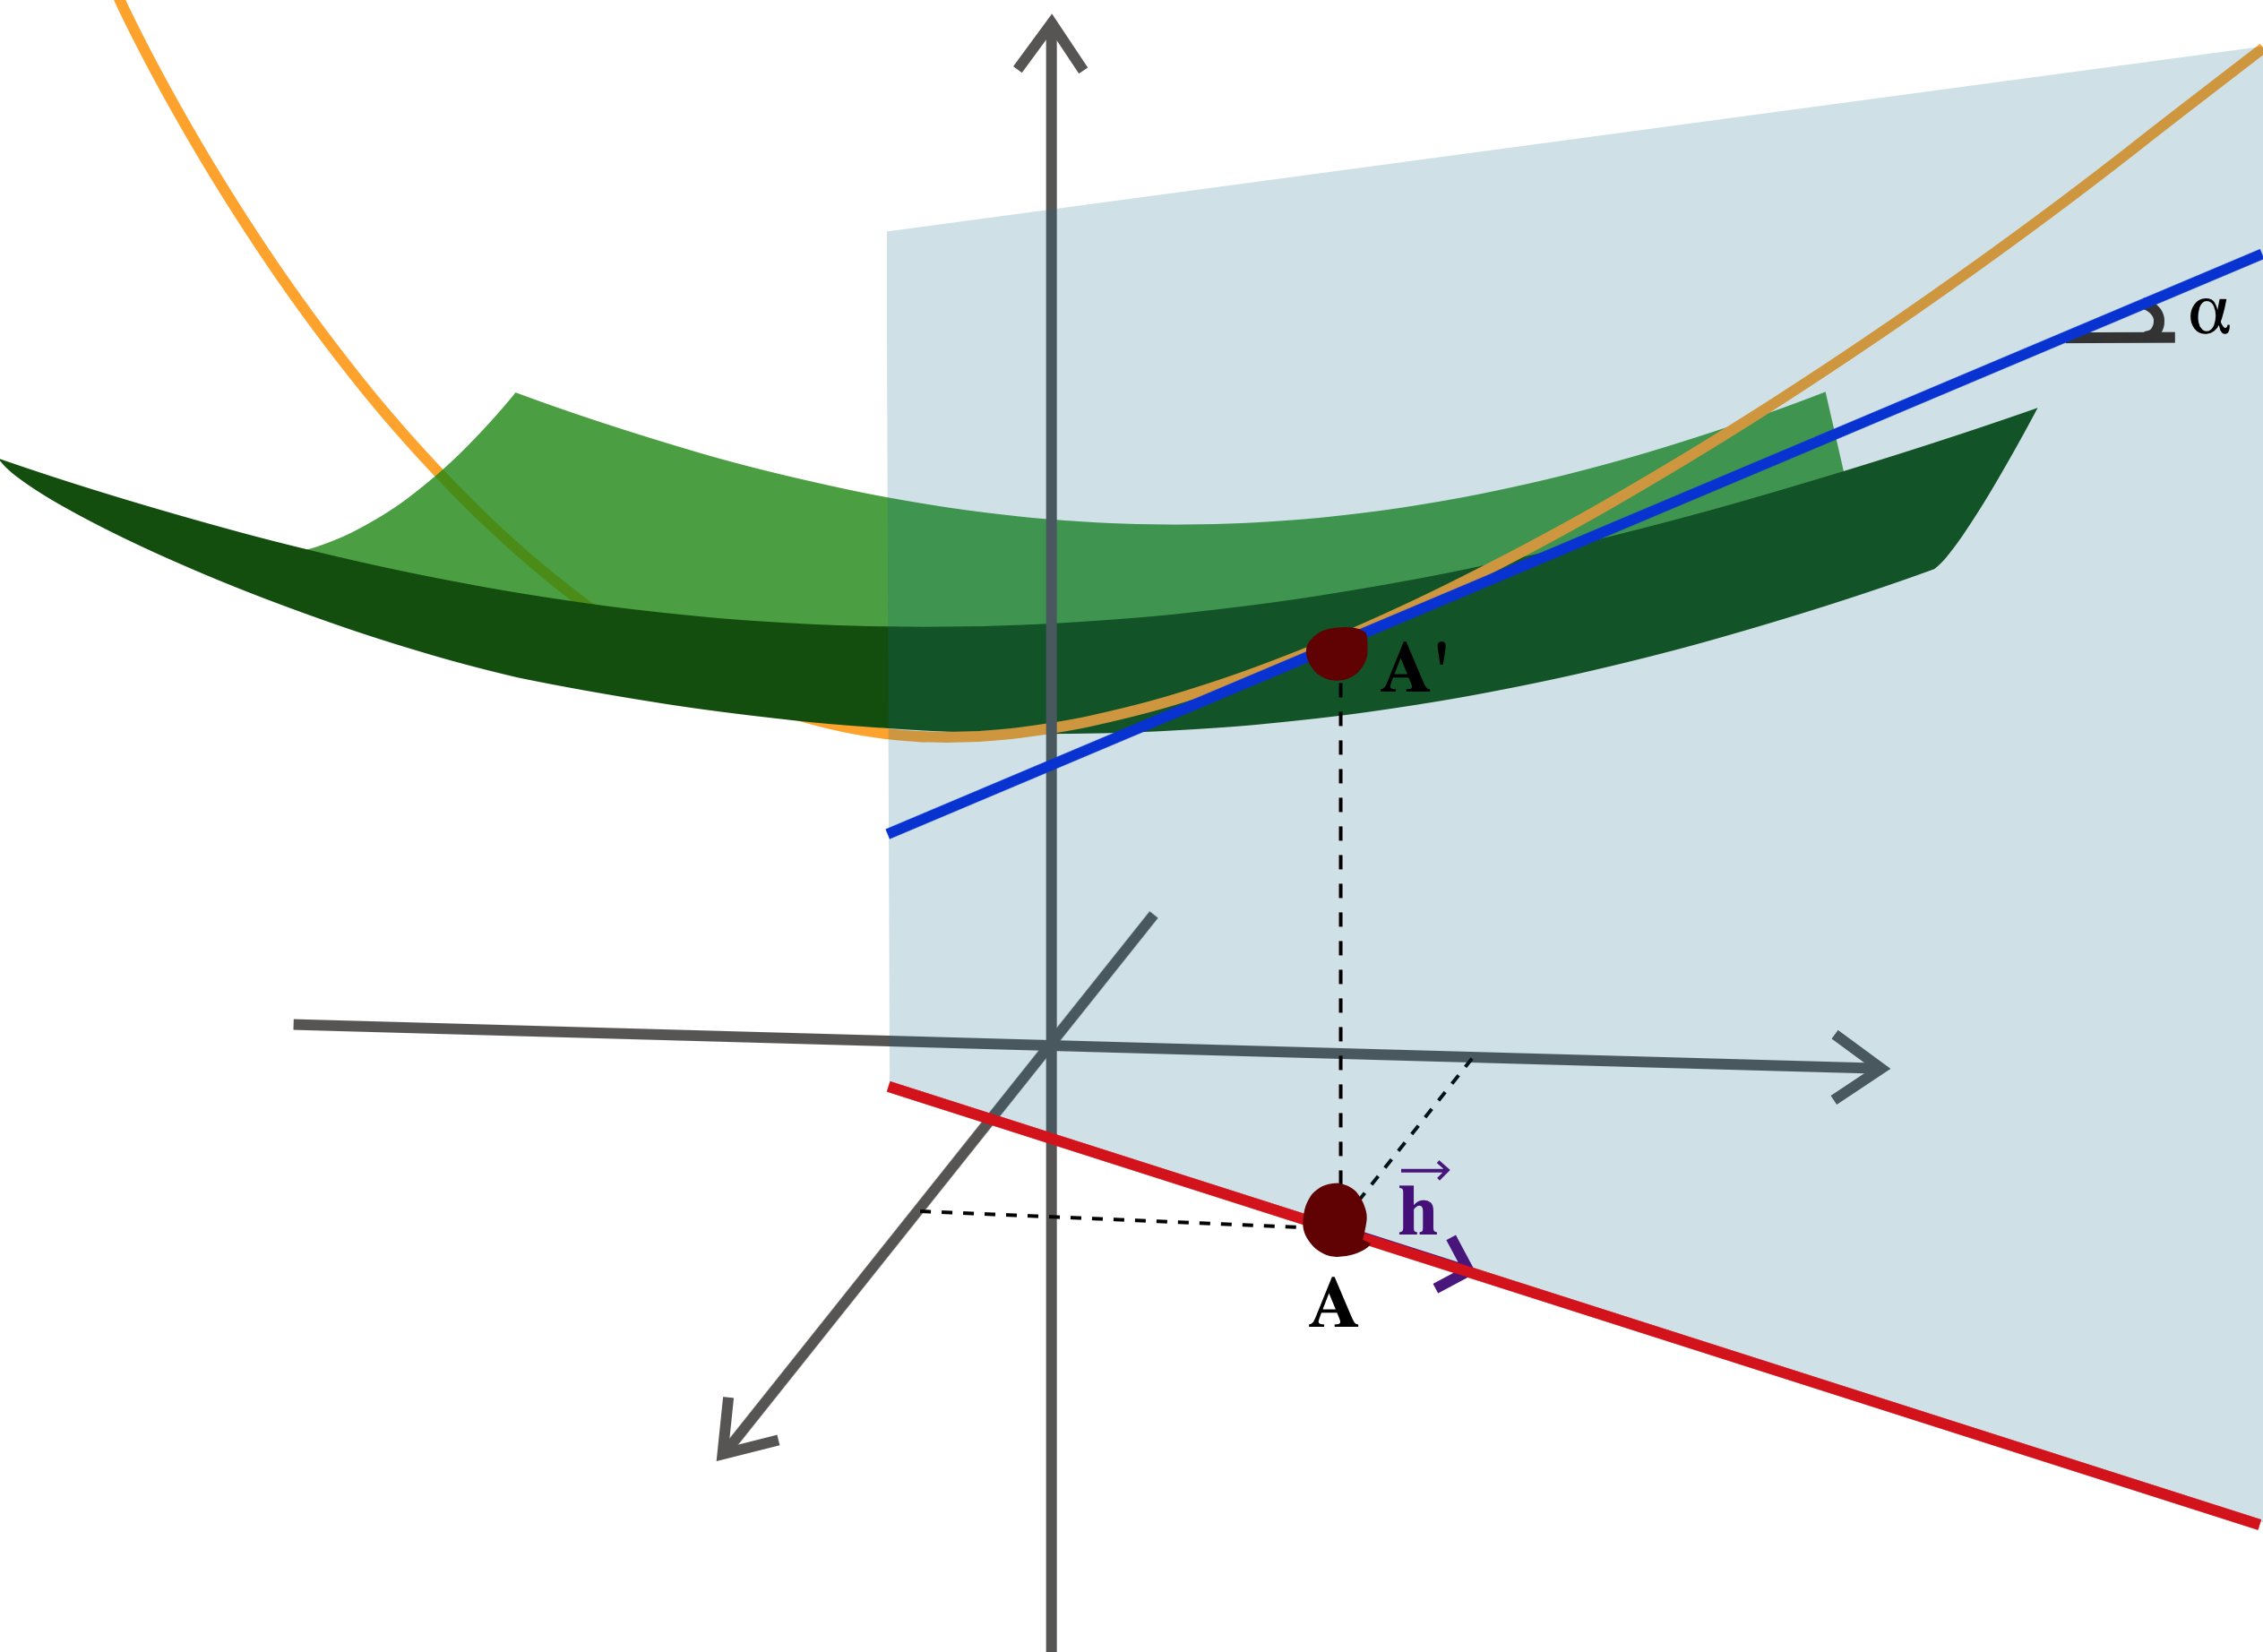
\includegraphics[width=0.5\hsize]{./figures-vectorcalc/directional-deriv.png}
 \end{figure} \pause
\begin{itemize}
\item Directional derivative should be zero \textit{in all directions} $\implies \diffF{f}{\vec x} = {\vec 0}$. \pause
\item For minimum: second directional derivative should be positive \textit{in all directions}.
\end{itemize}
\end{frame}


\begin{frame}{Summary}
Motivation: Want to optimise functions of several variables \\
\vspace{0.2cm}

% Q1: Understand how function changes when we change vector input. \\
% A1: Directional derivative, found from partial derivatives \\
% \vspace{0.2cm}

% Q2: 
\begin{itemize}
\item Directional derivative
\item Partial derivatives $\implies$ gradient vector
\item Steepest descent direction
\item At an optimum $\diffF{f}{\vec x} = \vec 0$
\end{itemize} \pause

\vspace{0.5cm}

Next time: Derivatives of vectors and chain rules.
\end{frame}





\end{document}

